% \documentclass[letterpaper]{article}

% \usepackage{natbib,alifeconf,amsmath,multirow,makecell,hyperref}  %% The order is important
% \usepackage[table]{xcolor}
% \usepackage{textcomp}
% \newcommand{\localapprox}{\raisebox{0.5ex}{\texttildelow}}


% *****************
%  Requirements:
% *****************
%
% - All pages sized consistently at 8.5 x 11 inches (US letter size).
% - PDF length <= 8 pages for full papers, <=2 pages for extended
%    abstracts (not including citations).
% - Abstract length <= 250 words.
% - No visible crop marks.
% - Images at no greater than 300 dpi, scaled at 100%.
% - Embedded open type fonts only.
% - All layers flattened.
% - No attachments.
% - All desired links active in the files.

% Note that the PDF file must not exceed 5 MB if it is to be indexed
% by Google Scholar. Additional information about Google Scholar
% can be found here:
% http://www.google.com/intl/en/scholar/inclusion.html.


% If your system does not generate letter format documents by default,
% you can use the following workflow:
% latex example
% bibtex example
% latex example ; latex example
% dvips -o example.ps -t letterSize example.dvi
% ps2pdf example.ps example.pdf


% For pdflatex users:
% The alifeconf style file loads the "graphicx" package, and
% this may lead some users of pdflatex to experience problems.
% These can be fixed by editing the alifeconf.sty file to specify:
% \usepackage[pdftex]{graphicx}
%   instead of
% \usepackage{graphicx}.
% The PDF output generated by pdflatex should match the required
% specifications and obviously the dvips and ps2pdf steps become
% unnecessary.


% Note:  Some laser printers have a serious problem printing TeX
% output. The use of ps type I fonts should avoid this problem.



%\title{Non-Epistatic Genetic Interactions Potentiate Exploration under Adaptive Momentum}
%\title{Adaptive Momentum Potentiates Evolutionary Exploration}
%\title{Predicting the Unpredictable: Using Replay Experiments to Isolate Changes in Adaptive Potential for Evolving Populations Outside of Equilibrium}
%\title{Predicting the Unpredictable: Using Replay Experiments to Isolate Changes in Evolutionary Potential for Non-equilibrium Populations}
%\title{Predicting the Unpredictable: Replay Experiments can Measure Changes in Evolutionary Potential during Disruptive Events}
%\title{Predicting the Unpredictable: Disentangling Long-Term Evolutionary Dynamics by using Replay Experiments to Measure Changes in Adaptive Potential}
%\title{Predicting the Unpredictable: Using replay experiments to disentangle how particular population dynamics affect evolutionary outcomes}
%\title{Predicting the Unpredictable: Using replay experiments to disentangle how evolutionary outcomes are altered by particular population dynamics}
%\title{Predicting the Unpredictable: Using replay experiments to disentangle how evolutionary outcomes are altered by adaptive momentum}
\chapter{Predicting the unpredictable: Using replay experiments to disentangle how evolutionary outcomes are altered by adaptive momentum}
\label{chap:adaptive_momentum}

\noindent
Authors: Austin J. Ferguson, Charles Ofria, and Clifford Bohm 

\noindent This chapter is adapted from a paper that has been peer-reviewed and accepted to appear in the proceedings of the 2024 Conference on Artificial Life. 

In this work we use the lens of historical contingency and potentiation to provide a new vantage point in understanding the adaptive momentum effect. 
According to the adaptive momentum framework, when a population is in disequilibrium some advantaged organisms can buffer more deleterious mutations than usual. 
This increased buffering increases evolutionary exploration until equilibrium is reestablished. 
Here we replay the evolution of select populations evolving in an idealized environment: a one-dimensional sawtooth function.
At each step we are able to quantify their potential to cross the next deleterious fitness valley. 
We find that populations experiencing disequilibrium, here caused by a selective sweep, see their potential to cross increase drastically with mutations near the leading edge of the sweep. 
Conversely, populations in equilibrium rely purely on chance to cross -- only the last mutations before a valley cross confer an increase in potential. 
Finally, we also performed ``shuffled'' replays to demonstrate that the structure of the population, not just its genetic makeup, is key in increased valley-crossing potential in this system. 

% KEY TERMS: Historical contingency, adaptive momentum, replay experiments, potentiation, disequilibrium, evolutionary dynamics, selective sweeps
%\author{}
%\author{Austin J. Ferguson$^{1,2,3,*}$, Charles Ofria$^{1,2,3}$, Clifford Bohm$^{3,4}$  \\
% \mbox{}\\
%  $^1$Department of Computer Science and Engineering
%  $^2$Program in Ecology, Evolution, and Biology\\
%  $^3$BEACON Center for the Study of Evolution in Action 
%  $^4$Department of Integrative Biology \\
%  Michigan State University, East Lansing, MI 48824 \\
% $^*$fergu358@msu.edu} % email of corresponding author


% For several authors from the same institution use the same number to
% refer to one address.
%
% If the names do not fit well on one line use
%         Author 1, Author 2 ... \\ {\Large\bf Author n} ...\\ ...
%
% If the title and author information do not fit in the area
% allocated, place \setlength\titlebox{<new height>} after the
% \documentclass line where <new height> is 2.25in



% \begin{document}
% \maketitle

% \begin{abstract}
% % Abstract length should not exceed 250 words
% % 210/250 words used
% (250 words max, shorter preferred).
When a new evolutionary dynamic is identified, researchers often struggle to understand its long-term effects on evolutionary outcomes.
Evolutionary prediction is always challenging, as subtle nuances of dynamics can interact in unpredictable ways.
Digital evolution systems, however, provide an empirical alternative to prediction: automated replay experiments can be conducted in large numbers to measure a real distribution of outcomes from a given starting point.
Changes in distributions over time can help us understand the long-term implications of seemingly minor events during evolution.
We apply this technique to ``adaptive momentum'', a new framework that explains how phenomena like selective sweeps can temporarily weaken selection and enhance the likelihood of crossing deleterious fitness valleys.
We show that deleterious mutations along the leading edge of a selective sweep can have an outsized influence on the evolutionary fate of a population.
Indeed, we see that evolutionary potential to cross new deleterious valleys drastically increases during selective sweeps.
Moreover, each valley crossing initiates a new sweep, increasing the potential for further discoveries; this increased potential subsides only once all sweeps have concluded.
While we still have much to learn about both adaptive momentum and the role of history in evolution, this work identifies important evolutionary dynamics at play and hones our tools for further studies.

% \end{abstract}

\section{Introduction}

% Innovations in science and technology periodically create opportunities to conduct experimental studies that were previously relegated to the realm of thought experiments. 
% This shift occurred with Stephen Jay Gould's idea of ``replaying the tape of life'' -- starting evolution over again to see if we would arrive at similar outcomes \citep{gouldWonderfulLifeBurgess1990}. 
% Previous researchers have brought this thought experiment into reality by leveraging microbial populations that can be frozen and then revived \citep{blountContingencyDeterminismEvolution2018} or digital populations that can be saved and loaded at will \citep{fergusonPotentiatingMutationsFacilitate2023}.
% By restarting evolution from different time points in an evolved population's history, researchers have begun to formalize \textit{analytic replay experiments} to test hypotheses on historical contingency.
% %Researchers have begun to leverage these \textit{analytic replay experiments} and the evolutionary counterfactuals they generate to test hypotheses on historical contingency.
% %Researchers have begun to leverage \textit{analytic replay experiments} where populations are restarted from particular time points to generate evolutionary counterfactuals and test hypotheses on historical contingency.
% Below we explore how these techniques can be expanded to develop a deeper understanding of evolutionary dynamics, in this case exploring the concept of ``adaptive momentum''.

% \subsection{Replay Experiments and Evolutionary Prediction}

% Traditional evolutionary biology is often focused on improving our ability to predict evolutionary outcomes or understand why evolutionary history played out the way it did.
% Prediction can be especially difficult in light of complex fitness landscapes with epistatic interactions, meaning that the result of mutational combinations cannot always be known based on individual effects.
% %, where one mutational event can change the impact of others, sometimes even making would-be deleterious mutations into beneficial ones.
% %Given the speed of modern digital evolution systems, however, we are able to shift from trying to simply predict evolution to empirically measuring the range and distribution of possible outcomes.
% Given the speed of digital evolution, however, we do not always need to predict evolutionary trajectories; we can often empirically measure the range and distribution of possible outcomes.
% % Further, by comparing the possible outcomes at different points in evolutionary history, we can determine how particular events influence the likelihood of different outcomes (i.e., historical contingency). 
% % These experiments/techniques allow us to refine our understanding of different dynamics and how they interact. 
% %Armed with not just what evolutionary endpoints were reached, but how particular events (even individual mutations) influenced which outcomes are more or less likely (i.e., historical contingency), we will be able to refine our understanding of different dynamics and how they interact.
% %Armed with not just evolutionary outcomes, but how particular events -- even individual mutations -- influence those outcomes (i.e., historical contingency), we can refine our understanding of different dynamics and how they interact.
% We can even directly measure historical contingency by conducting replay experiments before and after a particular event (such as one or more mutations).% to analyze the change in the distribution of outcomes.

% Thus far, these analytic replay experiments have been employed to study the genetic potentiation of complex traits, such as citrate metabolism in \textit{E. coli} \citep{blountHistoricalContingencyEvolution2008}, novel receptor usage in Phage $\lambda$ \citep{meyerRepeatabilityContingencyEvolution2012}, and associative learning in digital organisms \citep{fergusonPotentiatingMutationsFacilitate2023}.
% %Here we shift the focus from the evolution of a particular target trait and instead apply replay experiments to study fundamental evolutionary phenomena.
% Instead of focusing on the evolution of a particular target trait, here we apply replay experiments to an idealized model system to study fundamental evolutionary phenomena.
% %Instead of replaying the evolution of a particular complex trait, here we shift to a simplified model to use these techniques to better understand fundamental evolutionary phenomena. 

In Chapter \ref{chap:intro} we discussed how researchers are beginning to use analytic replay experiments to quantify how long-term evolutionary outcomes changed over the course of a population's history. 
Indeed, in Chapters \ref{chap:learning_case_studies} and \ref{chap:learning_distributions} we employed these replay techniques to identify key ``potentiating'' mutations in the evolution of associative learning in Avida. 
Here, we use these same replay techniques to understand the ``adaptive momentum'' effect \citep{Bohm2024.04.08.588357}.

Previously, replay experiments have been employed to measure the potentiation of complex traits and behaviors, both in microbial organisms \citep{blountHistoricalContingencyEvolution2008, meyerRepeatabilityContingencyEvolution2012, guptaHostparasiteCoevolutionPromotes2022, jochumsenEvolutionAntimicrobialPeptide2016a} and in digital organisms (Chapters \ref{chap:learning_case_studies} and \ref{chap:learning_distributions}).
Here we instead focus on the potentiation of a significantly simpler task: crossing deleterious fitness valleys in a one-dimensional sawtooth function. 
These fitness valleys require exactly six mutations to cross, which, due to the one-dimensional nature of this system, must be acquired in order. 
Therefore, we already know that any potentiating mutations must be a subset of these six mutations, and thus we are not searching for them as we were in the previous two chapters. 
However, we do not know the \textit{amount} of potentiation conferred by each of these six mutations. 
By comparing these potentiation dynamics of two categories of populations (those in disequilibrium and those in equilibrium), we can directly observe the effect that adaptive momentum has on evolutionary exploration and how these effects change over time. 

\subsection{Adaptive Momentum}

%Here, we use analytic replay experiments to study a newly identified dynamic called ``adaptive momentum'' \citep{Bohm2024.04.08.588357}.
The adaptive momentum framework suggests that periods of disequilibrium resulting from phenomena like selective sweeps and range expansions can enhance genetic exploration \citep{Bohm2024.04.08.588357}. 
We use analytic replay experiments to investigate this effect in selective sweeps.
Consider the appearance of a beneficial mutation in an asexual spatial population. 
If this mutation establishes and is sufficiently strong, it can trigger a selective sweep where the genotypes with the beneficial mutation come to dominate the population.
During the sweep, there will be a boundary between individuals with the beneficial mutation and those without (wild type).
If advantaged individuals along this boundary accrue relatively small deleterious mutations, they may still have a combined fitness benefit over the wild type. 
Thus, individuals along the leading edge of the sweep will have an increased potential to accumulate deleterious mutations that, in turn, increase the potential to explore genetic space and facilitate genetic discovery across fitness valleys. 
Adaptive momentum persists until the wild type is eradicated and equilibrium is reestablished. 
However, if during fixation a new beneficial mutation is discovered, the state of disequilibrium will persist, thus extending the ``momentum window'' (the period of adaptive momentum). 
\footnote{Adaptive momentum describes how disequilibrium during evolution can result in periods of increased mutation buffering. Such disequilibrium can be caused by several conditions, including sweeps, range expansions, and increases in carrying capacity in both spatial and well-mixed populations. The adaptive momentum framework further considers how the increased potential for mutational buffering can also affect large scale evolutionary rates via increased genetic exploration and subsequent genetic discovery.}


%These odds will remain elevated as long as sweeps continue and the population remains in fitness disequilibrium.
%Indeed, any type of fitness disequilibrium will initiate adaptive momentum, including environmental shifts, changes in population capacity, or even extinction events.
%In all cases adaptive momentum can result in beneficial mutations appearing in clustered groups.

In the work presented here, we create an ideal environment for adaptive momentum by using a one-dimensional spatial population evolving on a rising sawtooth fitness function.
%where each peak is higher than the previous, separated by a deleterious valley.
We use replay experiments to measure how the state of the population affects the potential to cross the next fitness valley. 
%We find that the effect of adaptive momentum is clearly visible in this simple system. 
Replay experiments show that %valley crosses are purely reliant on chance in populations not experiencing adaptive momentum. 
%However, 
%under the effect of 
adaptive momentum increases the potential for populations to cross fitness valleys, an effect that diminishes over time.
%Replay experiments show that valley crosses are purely reliant on chance, unless the population is experiencing adaptive momentum. 
%During adaptive momentum, populations see increased potential to cross fitness valleys, though that increase in potential diminishes over time. 
%Replay experiments show that valley crosses are pure chance when adaptive momentum is not in play, while populations experiencing adaptive momentum see increased potential to cross valleys, though that increase does diminish over time. 
%Further, we see that the leading edge of the selective sweep dictates the potential to cross early in the valley, though potential exceeds our expectations later in the valley.

Using simple assumptions about the structure of the leading edge of a selective sweep, we generated a predictive model of the potential for valley crossing during adaptive momentum. 
%This estimation is most accurate for early steps into the fitness valley, but loses accuracy when the leading edge is deeper in the valley and thus more stochastic events may have occurred, resulting in a higher state of disorder, which differs from the assumptions of the model.
While this estimation is highly accurate for early steps into the fitness valley, it loses accuracy when the leading edge is deeper in the valley. 
%This deviation from the predictive model is likely the result of historical contingency.
The time required for a population to reach deeper mutations in the fitness valley is likely also increasing the number of stochastic events that cause differences from the assumptions of the model. 
%The time required for a population to reach deeper mutations in the fitness valley increases the accumulation of stochastic events that increase its differences with the assumptions of the model. 
%This deviation from the predictive model is likely the result of accumulated stochastic events that have occurred in the path to reach deeper mutations in the fitness valley, resulting in a higher state of disorder and more differences with the assumptions of the model.
Finally, by shuffling organism positions in our population snapshots we can disrupt population structure.
This shuffled analysis allowed us to verify that the organization of the population, not just its genetic composition, is vital to valley-crossing potential. 
Overall, this work refines the framework proposed by adaptive momentum while advancing the methodology of analytic replay experiments as a tool for studying historical contingency, exposing sections of both that are ripe for further study. 




% \section{Introduction}

% Innovations in science and technology periodically create opportunities to conduct experimental studies that were previously relegated to the realm of thought experiments. 
% This shift occurred with Stephen Jay Gould's idea of ``replaying the tape of life'' -- starting evolution over again to see if we would arrive at similar outcomes \citep{gouldWonderfulLifeBurgess1990}. 
% Previous researchers have brought this thought experiment into reality by leveraging microbial populations that can be frozen and then revived or digital populations that can be re-instantiated at will.
% Researchers have begun to leverage these \textit{analytic replay experiments} and the evolutionary counterfactuals they generate to test hypotheses on historical contingency \citep{blountContingencyDeterminismEvolution2018}.
% Below we explore how these techniques can be expanded to develop a deeper understanding of evolutionary dynamics, in this case exploring the concept of ``adaptive momentum''.

% \subsection{Replay Experiments and Evolutionary Prediction}

% Thus far, analytic replay experiments have been employed to study the genetic potentiation of complex traits, such as citrate metabolism in \textit{E. coli} \citep{blountHistoricalContingencyEvolution2008}, novel receptor usage in Phage $\lambda$ \citep{meyerRepeatabilityContingencyEvolution2012}, and associative learning in digital organisms \citep{fergusonPotentiatingMutationsFacilitate2023} 
% (See \cite{blountContingencyDeterminismEvolution2018} for a review).
% Here we shift the focus from the evolution of a particular target trait and instead apply replay experiments to study fundamental evolutionary phenomena.

% Traditional evolutionary biology is often focused on improving our ability to predict evolutionary outcomes, or at least understand why evolutionary history played out the way it did.
% Prediction can be especially difficult in light of complex fitness landscapes with epistatic interactions, where one mutational event can change the impact of others, sometimes even making would-be deleterious mutations into beneficial ones.
% Given the speed of modern digital evolution systems, however, we are able to shift from trying to simply predict evolution to empirically measuring the range and distribution of possible outcomes.
% Armed with not just what evolutionary endpoints were reached, but how particular events (even individual mutations) influenced which outcomes are more or less likely (i.e., historical contingency), we will be able to refine our understanding of different dynamics and how they interact.

% \subsection{Adaptive Momentum}

% %Here, we use analytic replay experiments to study a newly identified dynamic called ``adaptive momentum'' \citep{Bohm2024.04.08.588357}.
% The adaptive momentum framework suggests that periods of disequilibrium resulting from phenomena like selective sweeps and range expansions can enhance genetic exploration \citep{Bohm2024.04.08.588357}. 
% We use analytic replay experiments to analyze this effect in selective sweeps.
% Consider the appearance of a beneficial mutation in an asexual spatial population. 
% If this mutation establishes and is sufficiently strong, it can trigger a selective sweep, a disequilibrium state, where the genotypes with the beneficial mutation come to dominate the population.
% During the sweep, there will be a boundary between individuals with the beneficial mutation and those without (wild type).
% If advantaged individuals along this boundary suffer relatively small deleterious mutations, they may still have a combined fitness benefit over the wild type. 
% The individuals along the leading edge of the sweep will have an increased potential to accumulate deleterious mutations that, in turn, increase the potential to explore genetic space, facilitating genetic discovery across fitness valleys. 
% Adaptive momentum persists until the wild type is eradicated. 
% However, if during fixation a new beneficial mutation is discovered, this will extend the ``momentum window'' (the period of adaptive momentum). 
% \footnote{In a most general sense, adaptive momentum describes how any disequilibrium conditions that arise during evolution will result in a period of increased mutation buffering. Adaptive momentum applies to several conditions, including sweeps, range expansions, and increases in carrying capacity in spatial and well-mixed populations. The adaptive momentum framework further considers how the increased potential for mutational buffering can also affect large scale evolutionary rates via changes to increased genetic exploration and subsequent genetic discovery.}


% %These odds will remain elevated as long as sweeps continue and the population remains in fitness disequilibrium.
% %Indeed, any type of fitness disequilibrium will initiate adaptive momentum, including environmental shifts, changes in population capacity, or even extinction events.
% %In all cases adaptive momentum can result in beneficial mutations appearing in clustered groups.

% In the work presented here, we create an ideal environment for adaptive momentum by using a one-dimensional spatial population evolving on a rising sawtooth fitness function.
% %where each peak is higher than the previous, separated by a deleterious valley.
% We use replay experiments to measure how the state of the population results in different potential to cross the next fitness valley. 
% %We find that the effect of adaptive momentum is clearly visible in this simple system. 
% Replay experiments show that %valley crosses are purely reliant on chance in populations not experiencing adaptive momentum. 
% %However, 
% under the effect of adaptive momentum, populations see an increased potential to cross fitness valleys that diminishes over time.
% %Replay experiments show that valley crosses are purely reliant on chance, unless the population is experiencing adaptive momentum. 
% %During adaptive momentum, populations see increased potential to cross fitness valleys, though that increase in potential diminishes over time. 
% %Replay experiments show that valley crosses are pure chance when adaptive momentum is not in play, while populations experiencing adaptive momentum see increased potential to cross valleys, though that increase does diminish over time. 
% %Further, we see that the leading edge of the selective sweep dictates the potential to cross early in the valley, though potential exceeds our expectations later in the valley.

% Using simple assumptions about the structure of the leading edge of a selective sweep, we generated a predictive model of the potential for valley crossing during adaptive momentum. 
% %This estimation is most accurate for early steps into the fitness valley, but loses accuracy when the leading edge is deeper in the valley and thus more stochastic events may have occurred, resulting in a higher state of disorder, which differs from the assumptions of the model.
% While this estimation is highly accurate for early steps into the fitness valley, it loses accuracy when the leading edge is deeper in the valley. 
% This deviation from the predictive model is likely the result of accumulated stochastic events that have occurred in the path to reach deeper mutations in the fitness valley, resulting in a higher state of disorder and more differences with the assumptions of the model.
% Finally, by shuffling organism positions in our population snapshots we can disrupt population structure.
% This shuffled analysis allowed us to verify that the organization of the population, not just its genetic composition, is vital to crossing potential. 
% Overall, this work refines the framework proposed by adaptive momentum while advancing the methodology of analytic replay experiments as a tool for studying historical contingency, exposing sections of both that are ripe for further study. 



\section{Methods}
% Here we describe the system used in this paper and detail the experiments conducted. 

\subsection{Evolution system}
% We used a minimal agent-based digital evolution model where each organism consists of a single integer genome, where fitness is determined as the expinentiation of the result of a sawtooth function based on genome value ($x$).
% To calculate fitness we first generate a score using a ``sawtooth'' function, similar to the one used by [CITE preprint], to create a landscape where local optima are separated by deleterious valleys.  
% Our sawtooth function (\(s\)) is defined as follows: 
% \[
% s(x) = kx - (k+d)(x\ \text{mod}\ w)
% \]
In order to isolate the adaptive momentum effect and keep computational costs feasible, we used a minimal agent-based evolution model where each organism's genome consists of a single integer, with value $x$. 
Fitness is based in a repeated ``sawtooth'' function, similar to the one used in \citep{Bohm2024.04.08.588357}, to create a landscape with regular fitness peaks separated by valleys. 
Each organism is assigned a quality score ($s(x)$), and then that score exponentiated to determine fitness ($f(x)=10^{s(x)}$). 
Score is calculated using the sawtooth function:

% \[
% s(x) = \frac{g}{w}x - (\frac{g}{w}+d)(x\ \text{mod}\ w)
% \]
\[
s(x) = \frac{x - (x~\text{mod}~w)}{w}G - (x~\text{mod}~w)D
\]

\noindent
where $G$ is the gain per peak, $D$ is the decrease per step into the valley, and $w$ is the valley width (number of mutational steps from one peak to the next). 
Effectively, the score function calculates the quality of the highest peak achieved and subtracts the cost of the current mutational step into the valley. 
%We used values of \(k = \frac{1}{6}\), \(a = w = 6\), and \(d = 0.05\).
We used $G=1.0$, $D=0.05$, and $w=6$.
This means that peaks appear every six steps; in this case at $x=6$, $x=12$, $x=18$, and so forth.
We refer to these peaks by their height, so those three peaks would be \(p_{1}\), \(p_{2}\), and \(p_{3}\), respectively.
We refer to the steps between peaks by the prior peak and an offset (\textit{e.g.}, $x=17$ is $p_{2} + 5$, the last step before $p_{3}$).
Figure \ref{fig-sawtooth} illustrates this sawtooth function and the relevant peaks.

Crossing a valley increases an organism's fitness by a factor of 10, and each step into the valley reduces fitness by \localapprox 12\%, relative to the previous peak. %regardless of which peak the organism was on.
We selected these drastic fitness differences to clearly demonstrate the effect.% rather than be representative of typical biological systems. 
%That being said, 
While this degree of selective benefit may be rare in biological systems, cases such as antibiotic resistance can show fitness increases of this magnitude \citep{gullbergSelectionResistantBacteria2011}.
%We stress that the degree of selective advantage modeled here may not represent typical biological systems.

\begin{figure}[h!]
\begin{center}
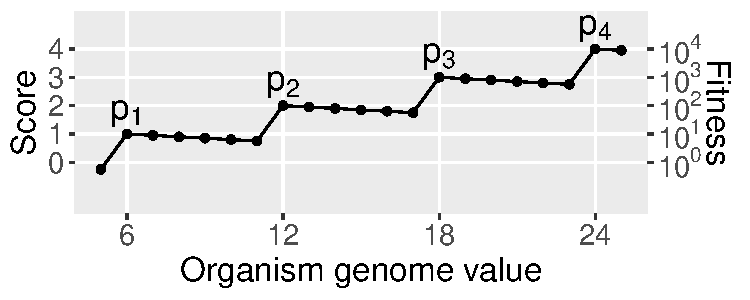
\includegraphics[width=0.75\textwidth]{05_adaptive_momentum/media/sawtooth_conceptual_figure.pdf}
\caption{
    The sawtooth function used in this work, with the four peaks mentioned in this work labeled.
    Score, $s(x)$, and fitness are both shown, with fitness being $10^{s(x)}$.
    %The function and parameters are available in methods. 
}
\label{fig-sawtooth}
\end{center}
\end{figure}

We evolved populations of 512 organisms in a one-dimensional spatial population -- a single line of organisms -- that did not wrap. 
This structure maximizes fixation times and makes selective sweeps easy to track, as they could only move left or right.
The population evolved via discrete, non-overlapping generations. 
%Each new generation of organisms was determined using spatial roulette (i.e., fitness-proportional) selection.%, where roulette selection was performed between the organism and its neighbors (for a maximum of three organisms per selection event). 
To fill positions in the next generation, we performed rounds of spatial roulette selection, each involving three organisms: the organism in that position in the previous generation and its two immediate neighbors (unless the organism is on the edge, in which case the roulette is between only two organisms). 
We then copied the selected individual to produce the offspring, with a $0.0125$ chance to mutate; mutations either increment or decrement the offspring's genome value by one. 
Selective sweeps are thus limited to advancing one position in the population per generation, limiting the growth rate and therefore the fixation time of a beneficial mutation. 
%When an organism is mutated, its integer value is incremented or decremented by one, and we used a mutation of rate of 0.0125 per reproduction event. 

\subsection{Experiment design}

We conducted this work in three stages: 
1) we validated that our model demonstrates adaptive momentum; 
2) we ran ``benchmarking'' data to create an expectation of how potentiation changes during a momentum window; 
and 3) we conducted analytic replay experiments to observe changes in potentiation in evolved lineages. 
Here we outline these experiments in more detail. 

\subsubsection{Experiment I: Model Validation}

%First, we wanted to ensure that our model allowed for valley crossing events, but for those events to be incredibly rare on their own. 
%To accomplish this, we ran 500,000 evolutionary replicates, where each replicate started with 512 organisms at $p_{2}$. 
%These replicates ran for 10,000 generations, much longer than the rest of our experiments, and we tracked the number of generations it took for the populations to cross the valley. 
%Some replicates crossed more than one valley, in which case we recorded the time since the previous crossing. 

%Additionally, we wanted to verify that disequilibrium is what drives the adaptive momentum effect. 

%The goal for our initial experiment was 
To ensure that our model could produce the adaptive momentum effect, 
%To do so, 
we replicated the primary experiment from \citep{Bohm2024.04.08.588357} comparing crossing times in populations starting from equilibrium versus those starting during the disequilibrium of a previous selective sweep. %were affected by the equilibrium state of a population.
We ran 500,000 evolutionary replicates, where each replicate started with 512 organisms at $p_{1}$ and ran for 5,000 generations. 
%, much longer than the rest of our experiments. 
%In the replicates where $p_{2}$ was discovered within in the first 5000 generations, we recorded the number of generations it took to discover $p_{2}$. 
In replicates where $p_{2}$ was discovered, we recorded the generation of discovery and extended the run duration for another 5,000 generations beyond the point of discovery. 
If $p_{3}$ was discovered before time ran out, we recorded this time as well. % to determine if and when $p_{3}$ was discovered. %In replicates that also discovered $p_{3}$, we recorded the number of generations between the discovery of $p_{2}$ and $p_{3}$ if that number was not greater than 5000. 
This methodology produced two time distributions: time to first crossing and time between first and second crossing, both capped at 5,000 generations.
%the first crossing time relative to the start time and the second crossing time relative to the first crossing time.

\subsubsection{Experiment II: Benchmarking}

%Adaptive momentum theory posits that organisms along the leading edge of a selective sweep experience reduced selection, and thus we expected valley crosses to be propelled by the leading edge. 
The adaptive momentum framework posits that populations in disequilibrium experience an increased rate of adaptation. % as long as the disequilibrium persists. 
In spatial populations experiencing a selective sweep, the disequilibrium should manifest near the leading edge of the sweep. 
Specifically, adaptive momentum allows deleterious mutations to accumulate within the advantaged subpopulation along the leading edge. 
This temporarily expanded mutant cloud increases genetic exploration, accounting for an observed increase in the rate of adaptation. 

\begin{figure}[h!]
\begin{center}
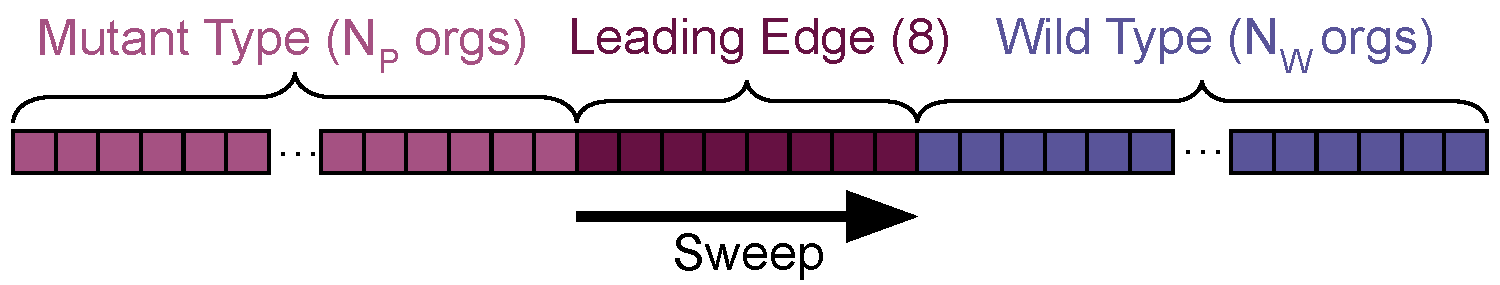
\includegraphics[width=0.85\textwidth]{05_adaptive_momentum/media/sweep_figure.pdf}
\caption{
    Starting layout for experiment II populations, with three clearly-defined sections: $N_P$ ``post-sweep'' mutant organisms at peak $p_{2}$ (left), $N_W$ ``wild type'' organisms at peak $p_{1}$ (right), and 8 ``leading edge'' organisms at a treatment-specific position in the valley past $p_{2}$ (middle).
}
\label{fig-experiment2}
\end{center}
\end{figure}

%We now explain how we apply potentiation to explore these claims.
We created idealized scenarios to study the dynamics of adaptive momentum as they unfold.
Each population had organisms on $p_{2}$ sweeping across organisms on $p_{1}$, with a well-defined leading edge (Fig. \ref{fig-experiment2}).
% of the sweep that are experiencing adaptive momentum.
%  and were experiencing high levels of purifying selection
% and were being swept away
Experimental treatments used all combinations of how far into the next fitness valley the leading edge started (from $x=p_{2}$ to $x=p_{2}+5$), and how far the sweep had progressed across the population (from $N_P=0$, at the beginning of a sweep, to $N_P=504$ at the end.)
%While the leading edge always consisted of eight organisms, its start ranged from position 0 (the beginning of a sweep with no post-sweep organisms) to 504 (the very end of a sweep with no wild-type left), with steps of eight.
%At each position, we tested the six sawtooth values that define a peak and the following valley, from $p_{2}$ to $p_{2} + 5$. 
%The leading edge was always initialized with eight organisms to ensure the post-sweep organisms did not immediately purify the leading edge.
We ran each replicate for $768-N_P$ total generations; the reduced number for larger $N_P$ was used to make the comparison fair, subtracting off the minimum time it could have taken to establish $N_P$ post-sweep organisms.
%, we assumed that if a leading edge is at position $n$ in the population, $n$ updates have already occurred. 
%For example, the replicates with an initial leading edge position of 256 only saw $768 - 256 = 512$ generations of evolution. 
For each condition, we measured how often replicates crossed the next valley to reach $p_{3}$.

We recorded the number of replicates that successfully crossed to $p_{3}$ in each treatment. 
This measurement provided an expectation of a population's potential to cross the valley \textit{based only on the initial state of the leading edge}.
Additionally, we also ran ``shuffled'' controls under otherwise identical conditions, but where we removed population structure (and thus the notion of a leading edge) by randomly shuffling the organisms before each evolutionary replicate.
%The shuffled benchmarks allowed us to evaluate if the population composition was sufficient to account for the results or if the spatial organization of the initialized population, consisting of a leading edge separating the purified post-sweep section from the wild type section, was also important.

\subsubsection{Experiment III: Analytic replays of evolved lineages}

Finally, we focused on the treatment from Experiment II that represented the start of a selective sweep; that is, no post-sweep organisms ($N_P=0$) and a leading edge that just made it to $p_{2}$. %peak 2 ($x=p_{2}$).
We ran 500 replicates under these conditions,
%initialized with the first eight organisms at $p_{2}$ and the rest at $p_{1}$, representing a population at the beginning of a selective sweep shortly after the discovery of a beneficial mutation.
%Again, these replicates evolved for 768 generations. 
saving snapshots at each generation, allowing us to perfectly recreate the population at any time point. 
We randomly selected 10 replicates that failed to reach $p_{3}$, 10 random replicates that did reach $p_{3}$ (but not further), and all four replicates that crossed two valleys to reach $p_{4}$.
For each of these 24 replicates, we performed 1000 analytic replays at every fourth generation, restarting evolution from a given time point with different random seeds to investigate the role of chance in determining \textit{the distribution of potential evolutionary outcomes} \citep{blountContingencyDeterminismEvolution2018}.
Next, we selected one representative sample from each of the three categories to study at high resolution, replaying 10,000 replicates from every generation. 

Using these replays, we recorded the probability that a replicate would cross the valley to $p_{3}$ or $p_{4}$ at each time point. 
These data allow us to calculate how the crossing probabilities changed over time. 
We also ran 10,000 equilibrium replicates and replayed representative replicates in the same manner. 
%This allows us to see how these probabilities changed over time, allowing us to see what generations were key for crossing -- or failing to cross -- that valley. 
%In addition, we recorded the same data for crossing a second valley (to $p_{4}$) in the same manner. 
Finally, just as in the shuffle benchmarking experiment, we performed ``shuffled'' replays on disequilibrium replicates that crossed a single valley.
Specifically, we shuffled the population before starting each replay to measure the role of the population's spatial organization in crossing potential. 

%[TODO - stats?]

\subsection{Data and software availability}
All code, analyses, summarized data, and figures not included in this work are available in the supplemental material \citep{austin_ferguson_2024_11507982}.
The model was built using the Modular Agent Based Evolver version 2.0 (MABE2) (\url{https://github.com/mercere99/MABE2}). 
All analyses and plots were generated using the R statistical computing language version 4.1.2 \citep{r_core_team_r_v4} and the ggplot2 \citep{R-ggplot2}, dplyr \citep{wickhamDplyrGrammarData2022}, HMisc \citep{harrelljrHmiscHarrellMiscellaneous2020}, tidyr \citep{wickhamTidyrTidyMessy2022} packages. %, and khroma \citep{frerebeauKhromaColourSchemes2023} packages. 








% \section{Methods}
% % Here we describe the system used in this paper and detail the experiments conducted. 

% \subsection{Evolution system}
% % We used a minimal agent-based digital evolution model where each organism consists of a single integer genome, where fitness is determined as the expinentiation of the result of a sawtooth function based on genome value ($x$).
% % To calculate fitness we first generate a score using a ``sawtooth'' function, similar to the one used by [CITE preprint], to create a landscape where local optima are separated by deleterious valleys.  
% % Our sawtooth function (\(s\)) is defined as follows: 
% % \[
% % s(x) = kx - (k+d)(x\ \text{mod}\ w)
% % \]

% We used a minimal agent-based evolution model where each organism's genome consists of a single integer, with value $x$. 
% Fitness is based in a repeated ``sawtooth'' function, similar to the one used in \citep{Bohm2024.04.08.588357}, to create a landscape with regular fitness peaks separated by valleys. 
% Each organism is assigned a quality score ($s(x)$), and then that score exponentiated to determine fitness ($f(x)=10^{s(x)}$). Score is calculated using the sawtooth function:

% % \[
% % s(x) = \frac{g}{w}x - (\frac{g}{w}+d)(x\ \text{mod}\ w)
% % \]
% \[
% s(x) = \frac{x - (x~\text{mod}~w)}{w}G - (x~\text{mod}~w)D
% \]

% \noindent
% where $G$ is the gain per peak, $D$ is the decrease per step into the valley, and $w$ is the valley width (number of steps from one peak to the next). 
% Effectively, the score function calculates the quality of the highest peak achieved and subtracts the cost of the current mutational step into the valley. 
% %We used values of \(k = \frac{1}{6}\), \(a = w = 6\), and \(d = 0.05\).
% We used values of $G=1.0$, $D=0.05$, and $w=6$.
% This means that we have peaks appear every six steps; in this case at $x=6$, $x=12$, $x=18$, and so forth.
% We refer to these peaks by their height, so those three peaks would be \(p_{1}\), \(p_{2}\), and \(p_{3}\), respectively.
% We refer to the steps between peaks by the prior peak and an offset (e.g., $x=17$ is $p_{2} + 5$; the last step before $p_{3}$).
% Figure \ref{fig-sawtooth} illustrates this sawtooth function and the relevant peaks.

% Crossing a valley increases an organism's fitness by a factor of 10, and each step into the valley reduces fitness by \localapprox 10\%, regardless of which peak the organism was on.
% We selected these drastic fitness differences to clearly demonstrate the effect rather than be representative of typical biological systems. 
% That being said, while this degree of selective benefit may be rare in biological systems, cases such as antibiotic resistance can show fitness increases of this magnitude \citep{gullbergSelectionResistantBacteria2011}.
% %We stress that the degree of selective advantage modeled here may not represent typical biological systems.

% \begin{figure}[h!]
% \begin{center}
% 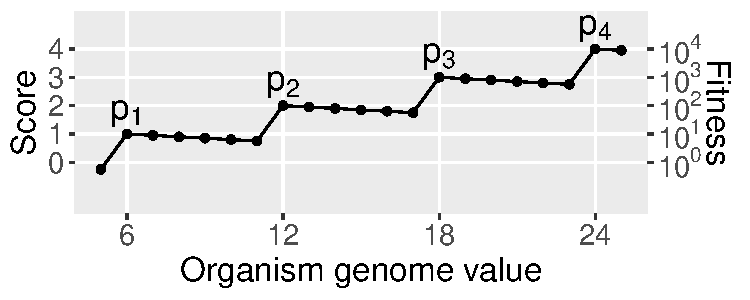
\includegraphics[width=0.75\textwidth]{05_adaptive_momentum/media/sawtooth_conceptual_figure.pdf}
% \caption{
%     The sawtooth function used in this work, with the four peaks mentioned in this work labeled.
%     Score, $s(x)$, and fitness are both shown, with fitness being $10^{s(x)}$.
%     %The function and parameters are available in methods. 
% }
% \label{fig-sawtooth}
% \end{center}
% \end{figure}

% We evolved populations of 512 organisms organized in a one-dimensional spatial population -- a single line of organisms -- that did not wrap. 
% This structure maximizes fixation times and makes selective sweeps easy to track, as they could only move left or right.
% The population evolved via discrete, non-overlapping generations. 
% %Each new generation of organisms was determined using spatial roulette (i.e., fitness-proportional) selection.%, where roulette selection was performed between the organism and its neighbors (for a maximum of three organisms per selection event). 
% To fill a position in the next generation, a round of spatial roulette selection was performed involving three organisms: the organism in that position in the previous generation and its two immediate neighbors (unless the organism is on the edge, in which case the roulette is between only two organisms). 
% The selected individual is then copied to produce an offspring. 
% This copy has a $0.0125$ chance to mutate, which will either increment or decrement the offspring's genome value by one. 
% Selective sweeps are thus limited to advancing one position in the population per generation, limiting the growth rate and therefore the fixation time of a beneficial mutation. 
% %When an organism is mutated, its integer value is incremented or decremented by one, and we used a mutation of rate of 0.0125 per reproduction event. 

% \subsection{Experiment design}

% We conducted this work in three stages: 
% 1) we validated that our model demonstrates adaptive momentum; 
% 2) we ran ``benchmarking'' data to create an expectation of how potentiation changes during a momentum window; 
% and 3) we conducted analytic replay experiments to observe changes in potentiation in the evolved lineages. 
% Here we outline these experiments in more detail. 

% \subsubsection{Experiment I: Model Validation}

% %First, we wanted to ensure that our model allowed for valley crossing events, but for those events to be incredibly rare on their own. 
% %To accomplish this, we ran 500,000 evolutionary replicates, where each replicate started with 512 organisms at $p_{2}$. 
% %These replicates ran for 10,000 generations, much longer than the rest of our experiments, and we tracked the number of generations it took for the populations to cross the valley. 
% %Some replicates crossed more than one valley, in which case we recorded the time since the previous crossing. 

% %Additionally, we wanted to verify that disequilibrium is what drives the adaptive momentum effect. 

% The goal for our initial experiment was to ensure that our model could replicate the adaptive momentum effect. 
% To do so, we replicated the primary experiment from \citep{Bohm2024.04.08.588357} to test whether crossing times were affected by the equilibrium state of a population.
% We ran 500,000 evolutionary replicates, where each replicate started with 512 organisms at $p_{1}$ and ran for 5,000 generations. 
% %, much longer than the rest of our experiments. 
% %In the replicates where $p_{2}$ was discovered within in the first 5000 generations, we recorded the number of generations it took to discover $p_{2}$. 
% In replicates where $p_{2}$ was discovered, we recorded the generation of discovery and extended the run duration for another 5,000 generations beyond the point of discovery. 
% If $p_{3}$ was discovered before time ran out, we recorded this time as well. % to determine if and when $p_{3}$ was discovered. %In replicates that also discovered $p_{3}$, we recorded the number of generations between the discovery of $p_{2}$ and $p_{3}$ if that number was not greater than 5000. 
% This methodology produced two time distributions: time to first crossing and time between first and second crossing, both capped at 5,000 generations.
% %the first crossing time relative to the start time and the second crossing time relative to the first crossing time.

% \subsubsection{Experiment II: Benchmarking}

% %Adaptive momentum theory posits that organisms along the leading edge of a selective sweep experience reduced selection, and thus we expected valley crosses to be propelled by the leading edge. 
% The adaptive momentum framework posits that populations in disequilibrium experience an increased rate of adaptation. % as long as the disequilibrium persists. 
% In spatial populations experiencing a selective sweep, the disequilibrium should manifest near the leading edge of the sweep. 
% Specifically, adaptive momentum allows deleterious mutations to accumulate within the advantaged subpopulation along the leading edge. 
% This temporarily expanded mutant cloud increases genetic exploration, accounting for an observed increase in the rate of adaptation. 

% \begin{figure}[h!]
% \begin{center}
% 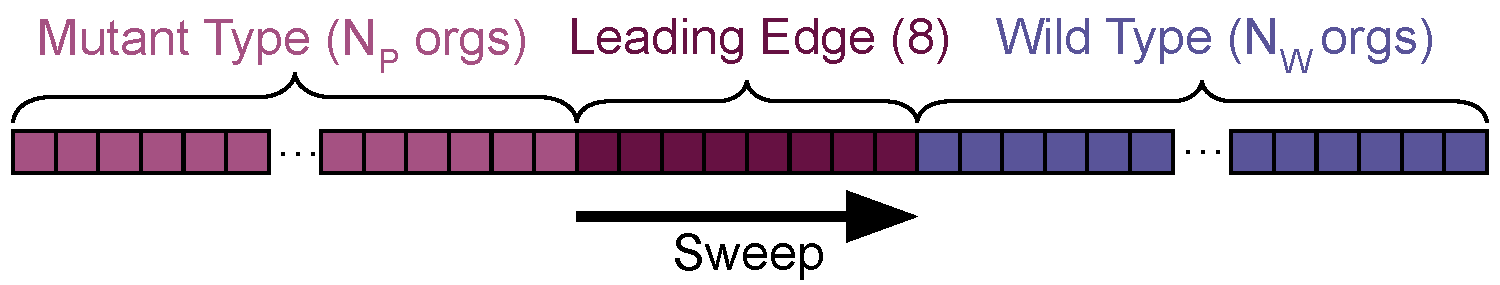
\includegraphics[width=0.85\textwidth]{05_adaptive_momentum/media/sweep_figure.pdf}
% \caption{
%     Starting layout for experiment II populations, with three clearly-defined sections: $N_P$ ``post-sweep'' mutant organisms at peak $p_{2}$ (left), $N_W$ ``wild type'' organisms at peak $p_{1}$ (right), and 8 ``leading edge'' organisms at a treatment-specific position in the valley past $p_{2}$ (middle).
% }
% \label{fig-experiment2}
% \end{center}
% \end{figure}

% %We now explain how we apply potentiation to explore these claims.
% We created idealized scenarios to study the dynamics of adaptive momentum as they unfold.
% Each population had organisms on $p_{2}$ sweeping across organisms on $p_{1}$, with a well-defined leading edge (Fig. \ref{fig-experiment2}).
% % of the sweep that are experiencing adaptive momentum.
% %  and were experiencing high levels of purifying selection
% % and were being swept away
% Experimental treatments used all combinations of how far into the next fitness valley the leading edge started (from $x=p_{2}$ to $x=p_{2}+5$), and how far the sweep had progressed across the population (from $N_P=0$, at the beginning of a sweep, to $N_P=504$ at the end.)
% %While the leading edge always consisted of eight organisms, its start ranged from position 0 (the beginning of a sweep with no post-sweep organisms) to 504 (the very end of a sweep with no wild-type left), with steps of eight.
% %At each position, we tested the six sawtooth values that define a peak and the following valley, from $p_{2}$ to $p_{2} + 5$. 
% %The leading edge was always initialized with eight organisms to ensure the post-sweep organisms did not immediately purify the leading edge.
% We ran each replicate for $768-N_P$ total generations; the reduced number for larger $N_P$ was used to make the comparison fair, subtracting off the minimum time it could take to establish $N_P$ post-sweep organisms.
% %, we assumed that if a leading edge is at position $n$ in the population, $n$ updates have already occurred. 
% %For example, the replicates with an initial leading edge position of 256 only saw $768 - 256 = 512$ generations of evolution. 
% For each condition, we measured how often replicates crossed the next valley to reach $p_{3}$.

% We recorded the number of replicates that successfully crossed to $p_{3}$ in each treatment. 
% This measurement provided an expectation of a population's potential to cross the valley \textit{based only on the initial state of the leading edge}.
% Additionally, we also ran ``shuffled'' controls under otherwise identical conditions, but where we removed population structure (and thus the notion of a leading edge) by randomly shuffling the organisms before each evolutionary replicate.
% %The shuffled benchmarks allowed us to evaluate if the population composition was sufficient to account for the results or if the spatial organization of the initialized population, consisting of a leading edge separating the purified post-sweep section from the wild type section, was also important.

% \subsubsection{Experiment III: Analytic replays of evolved lineages}

% Finally, we focused on the treatment from Experiment II that represented the start of a selective sweep; that is, no post-sweep organisms ($N_P=0$) and a leading edge that just made it to $p_{2}$. %peak 2 ($x=p_{2}$).
% We ran 500 replicates under these conditions,
% %initialized with the first eight organisms at $p_{2}$ and the rest at $p_{1}$, representing a population at the beginning of a selective sweep shortly after the discovery of a beneficial mutation.
% %Again, these replicates evolved for 768 generations. 
% saving snapshots at each generation, allowing us to perfectly recreate the population at any time point. 
% We randomly selected 10 replicates that failed to reach $p_{3}$, 10 random replicates that did reach $p_{3}$ (but not further), and all four replicates that crossed two valleys to reach $p_{4}$.
% For each of these 24 replicates, we performed 1000 analytic replays at every fourth generation, restarting evolution from a given time point with different random seeds to investigate the role of chance in determining \textit{the distribution of potential evolutionary outcomes} \citep{blountContingencyDeterminismEvolution2018}.
% Next, we selected one representative sample from each of the three categories to study at a higher resolution, replaying every generation for 10,000 replicates each. 

% Using these replays, we recorded the probability that a replicate would cross the valley to $p_{3}$ or $p_{4}$ at each of these time points. 
% These data allow us to calculate when and how the crossing probabilities changed over time. 
% We also ran 10,000 equilibrium replicates and replayed representative replicates in the same manner. 
% %This allows us to see how these probabilities changed over time, allowing us to see what generations were key for crossing -- or failing to cross -- that valley. 
% %In addition, we recorded the same data for crossing a second valley (to $p_{4}$) in the same manner. 
% Finally, just as in the shuffle benchmarking experiment, we performed ``shuffled'' replays on disequilibrium replicates that crossed a single valley.
% Specifically, we shuffled the population before starting each replay to determine the role of the population's spatial organization in crossing potential. 

% %[TODO - stats?]

% \subsection{Data and software availability}
% All code, analyses, summarized data, and figures not included in this work are available in the supplemental material \citep{austin_ferguson_2024_11507982}.
% The model was built using the Modular Agent Based Evolver version 2.0 (MABE2) (\url{https://github.com/mercere99/MABE2}). 
% All analyses and plots were generated using the R statistical computing language version 4.1.2 \citep{r_core_team_r_v4} and the ggplot2 \citep{R-ggplot2}, dplyr \citep{wickhamDplyrGrammarData2022}, HMisc \citep{harrelljrHmiscHarrellMiscellaneous2020}, tidyr \citep{wickhamTidyrTidyMessy2022} packages. %, and khroma \citep{frerebeauKhromaColourSchemes2023} packages. 

\section{Results}
%Below we describe the results in the same order the experiments were described, first validating the adaptive momentum effect, then moving onto benchmarking and replay experiment results.  

\begin{figure*}[h!]
\begin{center}
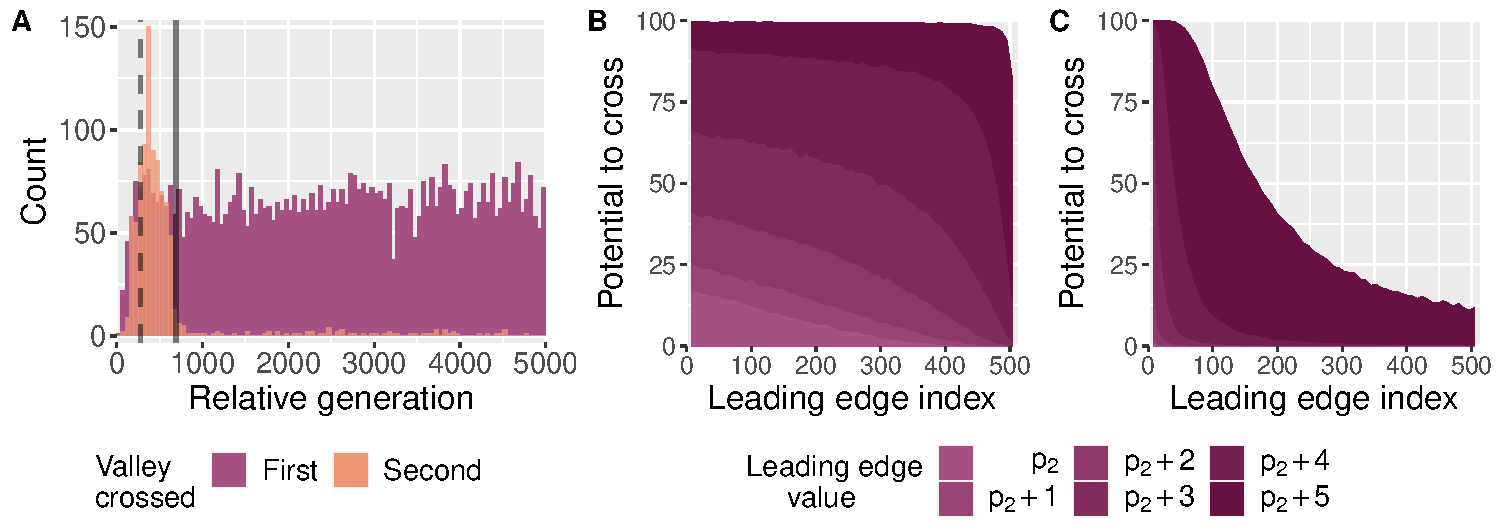
\includegraphics[width=\textwidth]{05_adaptive_momentum/media/combined_plots_full_split.pdf}
\caption{
    (A)
    Distribution of the number of generations required to cross valleys in the validation experiment. 
    Relative generations refer to the elapsed time (in generations) for the first cross (purple), and from the first cross to the second cross (orange). 
    %The solid and dashed horizontal lines show the expected count of first and second crosses per bar, respectively, for the expected uniform distribution. 
    The dashed and solid vertical lines show minimum and maximum fixation times, respectively. 
    (B) 
    Benchmarking data showing the potential of a leading edge to cross a valley, with a range of leading edge starting positions and values (see Fig. \ref{fig-experiment2}). 
    Each point represents 10,000 replicates.
    (C)
    Shuffled benchmarking data. Each replicate is shuffled prior to evolution, otherwise identical to center plot.
}
\label{fig-combined-plots}
\end{center}
\end{figure*}

\subsection{Validation of adaptive momentum effect}

First, we measured the time it took for replicates starting from a full population of $p_{2}$ to cross the valley to $p_{3}$ and, when relevant, from $p_{3}$ to $p_{4}$.
Figure \ref{fig-combined-plots}A
shows the timing distributions of populations that crossed the first valley over the first 5,000 generations (purple) as well as the timing distributions of second crossings that occur within 5,000 generations of a first (orange). 
We see that the time of first crossing appear uniformly distributed across the 5,000 generations, while the second crosses are strongly skewed toward shorter time periods. 
Indeed, of 500,000 replicates, 6,485 crossed the first valley within 5,000 generations (\localapprox 1.3\%) with a mean cross time of \localapprox 2,569 generations and a median of 2,602 generations. 
Based on these values, we would expect roughly 84 replicates to cross twice ($6,485 \times 1.3\%$, or 0.0169\% of all 500,000 replicates), but instead we see 902 replicates (\localapprox 0.18\%) cross the second valley, a much higher rate than expected if the probabilities of first and second crossing were equal.
In addition to a higher than expected rate of crossing, the mean cross time between first and second crossings is \localapprox 579 generations and the median cross time is 401 generations, substantially lower than the first crossing times. 
Finally, when we consider only those second crossing times that occurred more than 1000 generations after a first crossing, we find that the rate of these second crossings is similar to the first crossing rate (\localapprox 1.23\%).
These results comport with the framework of adaptive momentum. 
They show that an initial beneficial discovery can quickly lead to additional discoveries (during the fixation period), but if the second discovery does not happen before equilibrium is reestablished, the rate of valley crossing is better predicted by the first valley crossing times. 


% Indeed, of 500,000 replicates, 12,793 crossed at least once (\localapprox 2.6\%) with a mean cross time of \localapprox 4,995 generations and a median of 4,951 generations. 
% We would expect that only 338 replicates to cross twice (2.6\% squared), but instead we see 1,734 replicates cross at least two valleys (\localapprox 0.35\% of total, or \localapprox 13.6\% of those that crossed once). 
% For the second crossings, we see a mean cross time of 646 generations and a median cross time of 396 generations. 
% Indeed, while not shown in Figure \ref{fig-crosses-from-scratch}, we see 200 replicates cross at least three valleys, 26 replicates cross at least four valleys, and six replicates cross five valleys; of these higher-order crossings, the median time to cross was always less than 420 generations. 
% These findings, where an initial beneficial discovery can quickly lead to additional discoveries, supports the initial adaptive momentum theory. 

% \begin{figure}[h!]
% \begin{center}
% 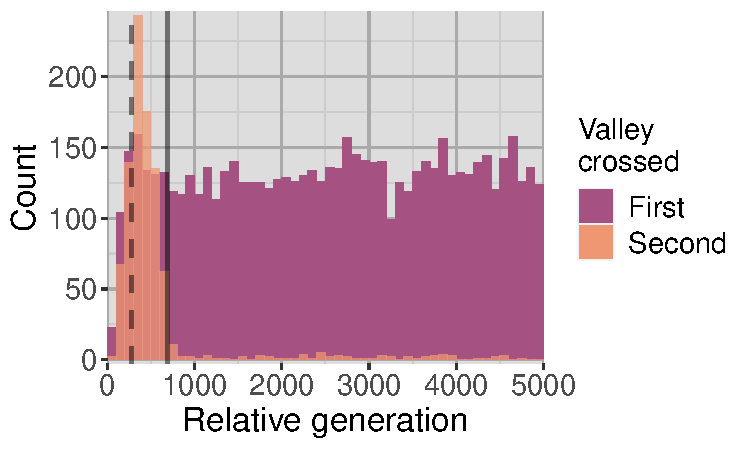
\includegraphics[width=0.45\textwidth]{media/first_two_crosses_overlayed_fair_comparison_with_fixation.pdf}
% \caption{
%     Distribution of the number of updates required to cross valleys in the validation experiment. 
%     Relative updates refer to the number of elapsed generations for the first cross, and the number of generations since the first cross for the second cross. 
%     %The solid and dashed horizontal lines show the expected count of first and second crosses per bar, respectively, for the expected uniform distribution. 
%     The dashed and solid vertical lines show the minimum and maximum fixation times, respectively. 
% }
% \label{fig-crosses-from-scratch}
% \end{center}
% \end{figure}





%Further, we tested the role of disequilibrium in these discoveries by comparing the evolution of populations seeded with eight organisms on $p_{2}$ and the rest on $p_{1}$ (disequilibrium treatment) against whole populations of $p_{2}$ (control). 
%We found that 1,751 of 10,000 disequilibrium replicates crossed the first valley (\localapprox 17.5\%), while only 23 of 10,000 control replicates crossed (\localapprox 0.2\%). 
%This difference is highly significant ($p < 10^{-15}$, Fisher's exact test).
%This further supports the claim that adaptive momentum relies on disequilibrium in the population, and shows that we can start artificially start an adaptive momentum window in this system by creating this disequilibrium. 

\subsection{Empirical benchmarks}

%After confirming that disequilibrium can facilitate valley crosses, we next tested idealized populations to benchmark the effect on valley crossing of two components of this disequilibrium: the position of the leading edge, and the genotypes of the organisms comprising that leading edge.
The empirical benchmark data (Fig. \ref{fig-combined-plots}B) illustrate how the initial state of the population affects the potential to cross valleys.
%In particular the ratio of the population initiated on $p_2$ (mutant type), versus $p_1$ (wild type) and the value of the individuals on the leading edge,
As expected, steps further into the valley increase the probability of crossing, regardless of where the leading edge is. 
On the other hand, the probability of crossing decreases as the ratio of $p_2$ organisms (mutant type) increases relative to $p_1$ organisms (wild type) -- as the selective sweep progresses, fewer opportunities remain for additional mutations to accumulate. 
While the potential to cross varies considerably with the type of organisms in the leading edge, these data clearly show that all conditions describing early sweep conditions (\textit{i.e.}, having a leading edge and a significant ratio of the remaining population on $p_1$) %having any leading edge 
substantially increase the probability of crossing the valley compared to populations that are close to reaching equilibrium on $p_2$. 

%The benchmarks with a leading edge at index 0 see slightly lower rates of crossing, as they only have one organism at the given value while every other point has 8 organ
%We typically ran these benchmarking populations with a leading edge of eight organisms of the same type to remove the possibility of genetic drift immediately destroying the leading edge. 
%This drift accounts for the drop in crosses at index 0, the one instance where the leading edge consisted of only a single organism. 
%Finally, being one step away from crossing the valley ($p_2$ + 5) effectively guarantees a cross, as eight organisms at that value are almost certain to accumulate the one needed mutation unless the selective sweep is almost over. 
%Overall, these data match our expectations. 
We use these results to provide a baseline prediction for the analytic replay experiments. 

% \begin{figure}[h!]
% \begin{center}
% 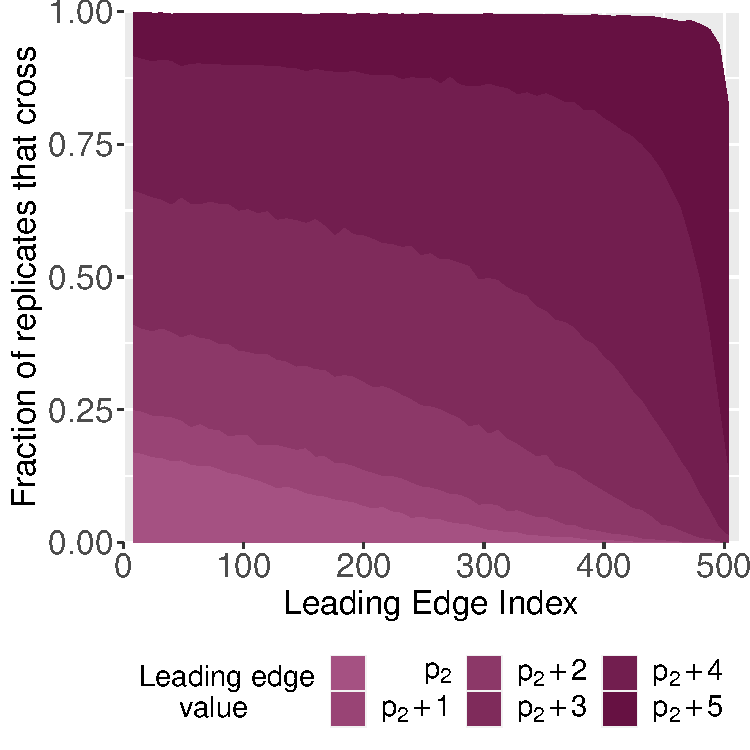
\includegraphics[width=0.45\textwidth]{media/benchmarking_area.pdf}
% \caption{
%     Benchmarking data showing the potential of a leading edge to induce a valley cross, with a range of leading edge values and starting positions. 
%     The leading edge always consists of eight organisms of that value. 
%     Each point represents 10,000 replicates. 
% }
% \label{fig-benchmarking}
% \end{center}
% \end{figure}

\subsection{Analytic replay experiments}
Of our 500 initial replicates to find candidates for replay experiments, four replicates (0.8\%) crossed two valleys in the allotted time, 83 crossed exactly one valley (16.6\%), and the remaining 413 did not cross any valleys (82.6\%). 
%We ran coarse-grained replays for 10 randomly-sampled no-cross replicates, 10 random single-cross replicates, and all four double-cross replicates.
We randomly-sampled 10 no-cross replicates, 10 single-cross replicates, and took all four double-cross replicates to run coarse-grained replays.
%We ran coarse-grained analytic replay experiments for all four replicates that crossed twice and for 10 randomly-sampled replicates of each of the two other categories. 
%For each of these 24 replicates, we replayed at every fourth generation, with 1,000 replicates per time point. 
All plots are available in the supplement \citep{austin_ferguson_2024_11507982}. 

From these coarse-grained replays, we selected one representative replicate from each category to re-run, conducting 10,000 replay trials at \textit{every} time point to give a fine-grained view. 
%We show the replay results in two formats. 
%The first showing the potential of crossing the next valley over time and the second as Muller plots showing the underlying population structure that beget that potentiation. 
For each replayed replicate, we show the potential of crossing the next valley over time, paired with a Muller plot \citep{mullerGeneticAspectsSex1932} of the initial replicate that was replayed. 
Figures \ref{fig-replay-single-cross}, \ref{fig-replay-double-cross}, and \ref{fig-replay-no-cross} show the single-cross, double-cross, and no-cross replicates, respectively. 
%In each plot, the replay results are overlaid atop the benchmarking data, which has been adjusted such that the leading edge index aligns with the actual leading edge at that generation of the population.
In each plot, the replay results are overlaid on an image generated from the benchmark data. 
%To generate the background image, we treat the benchmark data as a lookup function and use the current position of the leading edge of the replay result to look up the potentiation predicted by the benchmark data. 
To generate the background image, we treat the benchmark data as a lookup function.
When we start a replay replicate, we initialize the population using the snapshot from the target generation of the initial replicate. 
These snapshots show that the leading edge does not perfectly advance one position every generation; there are many generations where the leading edge either fails to advance or is pushed back one position by the wild type organisms.
%As we see in our population snapshots, the leading edge does not actually advance one position every generation, the leading often fails to advance, and occasionally the wild-type organisms replicate over the leading edge, pushing it back one step. 
To make this comparison fair, we find the leading edge in that particular snapshot and then look up the corresponding expectation values from the benchmark data. 
%Thus, the background image shows in ``real time'' potentiation of the replay at each generation.
This adjustment ensures that we are comparing against the correct benchmark data regardless of the motion of the leading edge. 
%Thus, the background image adjusts 

Overall, the potentiation observed in all three replicates closely match the benchmark expectations. 
The potentiation occasionally increases or decreases suddenly; tracing these changes to the Muller plots typically shows that these events correlate to the gain or loss of a mutation at (or near) the leading edge at that time. 
For example, the two temporary peaks in potential in Figure \ref{fig-replay-single-cross}, at roughly generations 250 and 375, can be directly traced to the leading edge temporarily dipping to $p_{2} + 4$.
%When the leading edge mutates further into the fitness valley, the potentiation increases dramatically. 
%Each of the three replicates 
The potentiation at any particular step in the valley decreases over time, as the selective sweep progresses and the adaptive momentum window closes.
Figure \ref{fig-replay-no-cross} shows that, while the replicate had substantial potentiation at times (briefly above 50\%), it failed to capitalize before the window closed. 
This failure was exacerbated by two leading mutations from $p_{2} + 3$ to $p_{2} + 2$, the second of which dropped the potential from over 25\% to under 10\%, after which the population never recovers. 
% It should be noted that the dramatic increases or decreases in potentiation can be mapped cleanly onto the Muller plots showing the state of the population. 
% For example, in Figure \ref{fig-replay-single-cross} potentiation temporarily increases dramatically (from \localapprox 60\% to \localapprox 90\%) twice, once around update 250 and again around update 350. 
% In both cases, the potentiation then drops to previous levels shortly after. 
% Mapping this points onto the Muller plot, we see that, in both cases, the leading edge drifted down an additional step into the valley (to $p_{1} + 4$) before quickly drifting back to the previous step. 
% These drops in potentiation are particularly dramatic in the no-cross replicate of Figure \ref{fig-replay-no-cross}, where a late drift backward reduces the potential to cross from over 25\% to under 10\%, from which the population never recovers. 

All three replicates show periods of potentiation higher than what our benchmark data would predict given their leading edge genomic value. 
The benchmarking data modeled a leading edge of eight organisms, but the Muller plots show that the leading edge grows and shrinks over time. 
The Muller plots show that underprediction is generally associated with either an expanded leading edge or an excess of individuals with lower fitness behind the leading edge. 
We hypothesize that these underpredictions are generally observed in deeper steps into the valley because of the historical contingency required to reach that point (\textit{i.e.}, to reach $p_{2} + 5$ the leading edge must have passed through $p_{2} + 4$, which may still exist behind the leading edge).
%While all organisms behind the leading edge are experiencing purifying selection, this purification takes time, and a cluster of mutated organisms can persist behind the leading edge. 
%Our benchmark expectations are particularly accurate for early steps into the valley; even if a large cluster of organisms exists behind the leading edge, they are still unlikely to accumulate the needed mutations to cross the valley before being purified. 
%In contrast, when the leading edge is only a mutation or two away from crossing, even a few organisms trailing the leading edge can be enough to cross the valley. 
%If a sizable section of the population is only two or three mutations from crossing the valley, the size of that section may buffer the organisms from purifying selection long enough for some organisms to genetically drift to the next peak. 
%This is supported by the replays almost perfectly aligning with the expectation in the first few steps into the valley, where the mutation rate cannot outpace the rate of purifying selection, while the empirical potentiation is often above the expectation in the last few steps of the valley. 
%This was not explicitly modeled in the benchmarking data, possibly causing this difference. 
%while replays see leading edges that are much larger or smaller, causing some variation from the expectation.
%Further, our benchmarks are based \textit{only} on the leading edge, and thus our hypothesis is that this higher-than-expected potentiation results from the evolutionary potential of non-leading edge organisms. 

\begin{figure}[h!]
\begin{center}
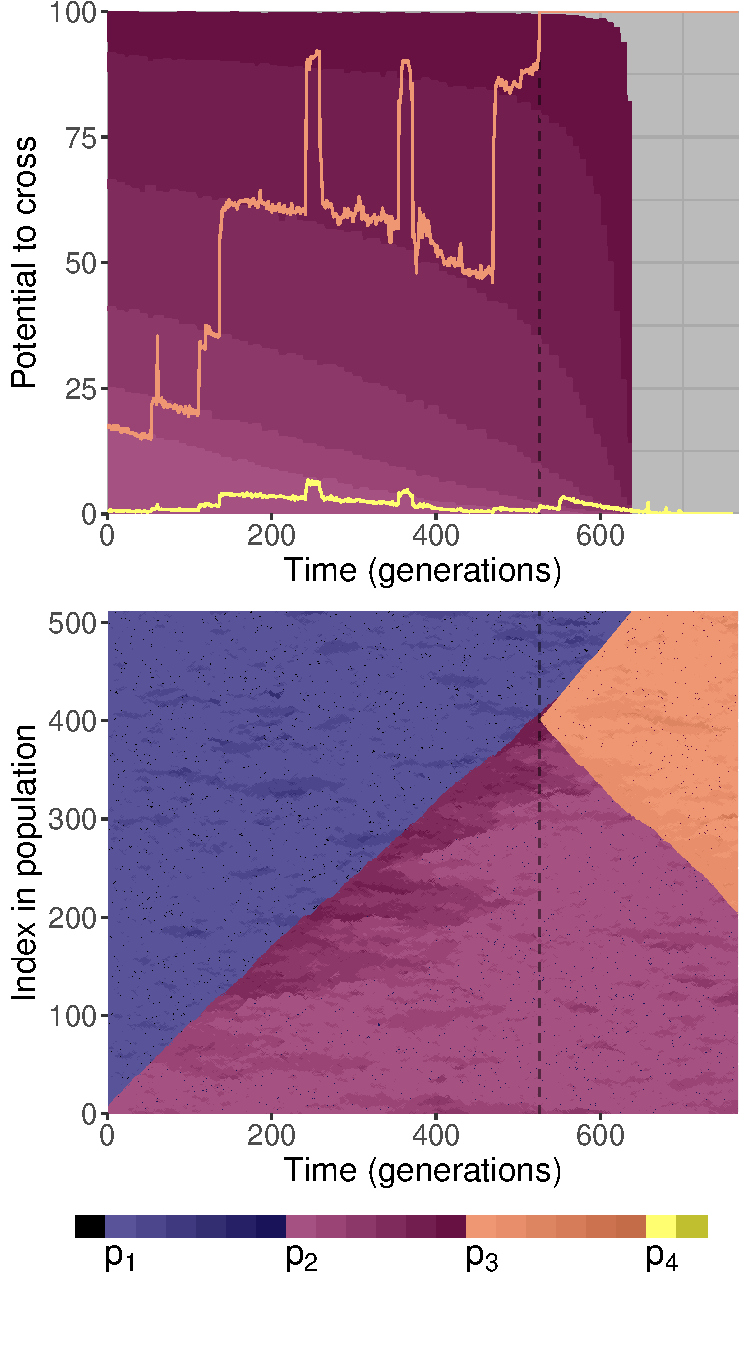
\includegraphics[width=0.6\textwidth]{05_adaptive_momentum/media/reps/400/script_06__plot_05__combined_plot_area_palette.pdf}
\caption{
    Top plot: Analytic replay data for a representative replicate that crossed one valley during a momentum window, overlayed on baseline data. 
    Lines show the probability of crossing both the first valley  (orange line; initially-higher) and the second valley (yellow line; initially-lower). 
    The background shows the expected potential to cross (as shown in Fig. \ref{fig-combined-plots}B); data here are shifted to align with the realized leading edge position. 
    %Each update was replayed 10,000 times. 
    Bottom plot: A Muller plot of all organisms in the original 1D population over time. 
    Dark colors show descent into valleys, with hue identifying the valley being crossed. 
    In both plots, vertical dashed lines show initial valley crosses.
    Colors in the legend apply to all plots. 
}
\label{fig-replay-single-cross}
\end{center}
\end{figure}

\begin{figure}[h!]
\begin{center}
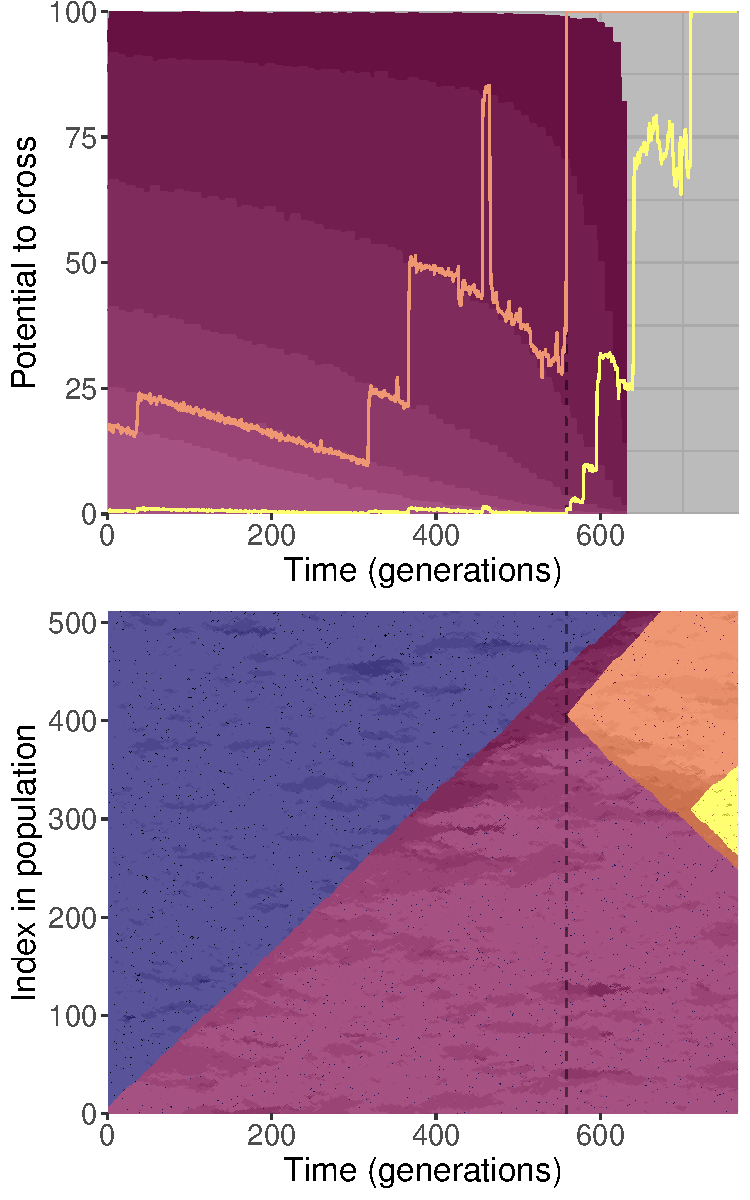
\includegraphics[width=0.6\textwidth]{05_adaptive_momentum/media/reps/263/script_06__plot_03__combined_plot_area.pdf}
\caption{
    The analytic replay data for a representative replicate that crossed two valleys during a momentum window. 
    See Figure \ref{fig-replay-single-cross} for details and legend. 
}
\label{fig-replay-double-cross}
\end{center}
\end{figure}

\begin{figure}[h!]
\begin{center}
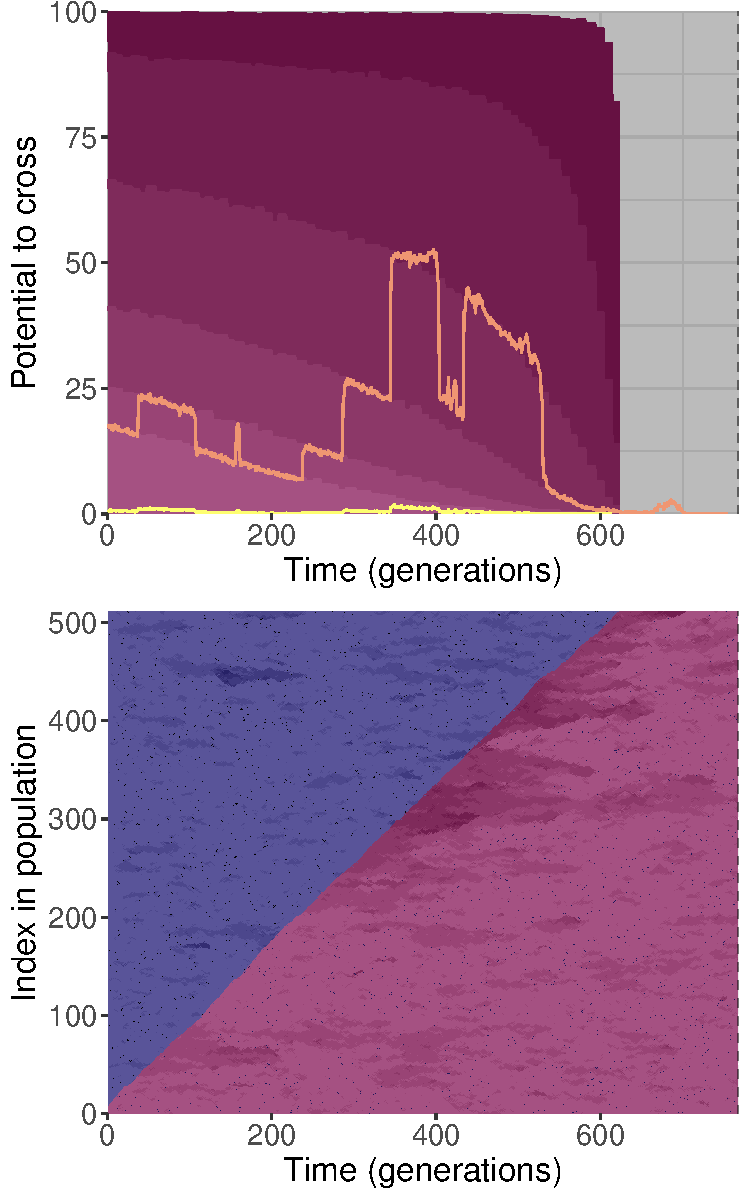
\includegraphics[width=0.6\textwidth]{05_adaptive_momentum/media/reps/339/script_06__plot_03__combined_plot_area.pdf}
\caption{
    The analytic replay data for a representative replicate that failed to cross a valley during a momentum window.
    See Figure \ref{fig-replay-single-cross} for details and legend.
}
\label{fig-replay-no-cross}
\end{center}
\end{figure}

For comparison, we also ran 10,000 replicates that started at equilibrium (\textit{i.e.}, not in a momentum window).
Of those, we replayed the one replicate that crossed twice, 10 randomly sampled replicates from 19 that crossed once, and 10 random replicates from the 9,980 that failed to cross. 
Figure \ref{fig-replay-no-window} shows the replicate that crossed twice. 
The first crossing in this replicate occurred quite early, crossing the valley on generation 168. 
However, the potential before crossing is similar to all first-cross replicates: while the potential in an adaptive momentum window starts at \localapprox 17\%, the potential for replicates outside momentum windows starts at \localapprox 0.2\%. 
This low potential continues for the first 143 generations, followed by 16 generations with an average potential of \localapprox 1.8\%, four generations between 15\% and 20\%, and then the cross. 
%This pure chance, ``all or nothing'' potentiation is not unique to this replicate, as we see in the histograms of potential shown in Figure \ref{fig-histograms}.
This pure chance, ``all or nothing'' potentiation is not unique to this replicate; the same dynamic can be seen in the ten other successful replicates we analyzed \citep{austin_ferguson_2024_11507982}.
% Figure \ref{fig-replay-no-window} shows the potential for the first and second valley crossing. 
% The potential for the first valley crossing remains very low ($<$0.4\%) until it increased to 100\% in less than 20 generations. 
% This increase is not linear, however, as there is an initial increase and then a drop in potentiation, likely corresponding to the flux in $p_{2} + 5$ organisms in the population. 
% The discovery of $p_{3}$ starts a momentum window, and the potential of the second cross then looks like the potential in previous results (although limited by the lack of remaining time), and is higher than the potential of the first window was for the first \localapprox 580 generations.


\begin{figure}[h!]
\begin{center}
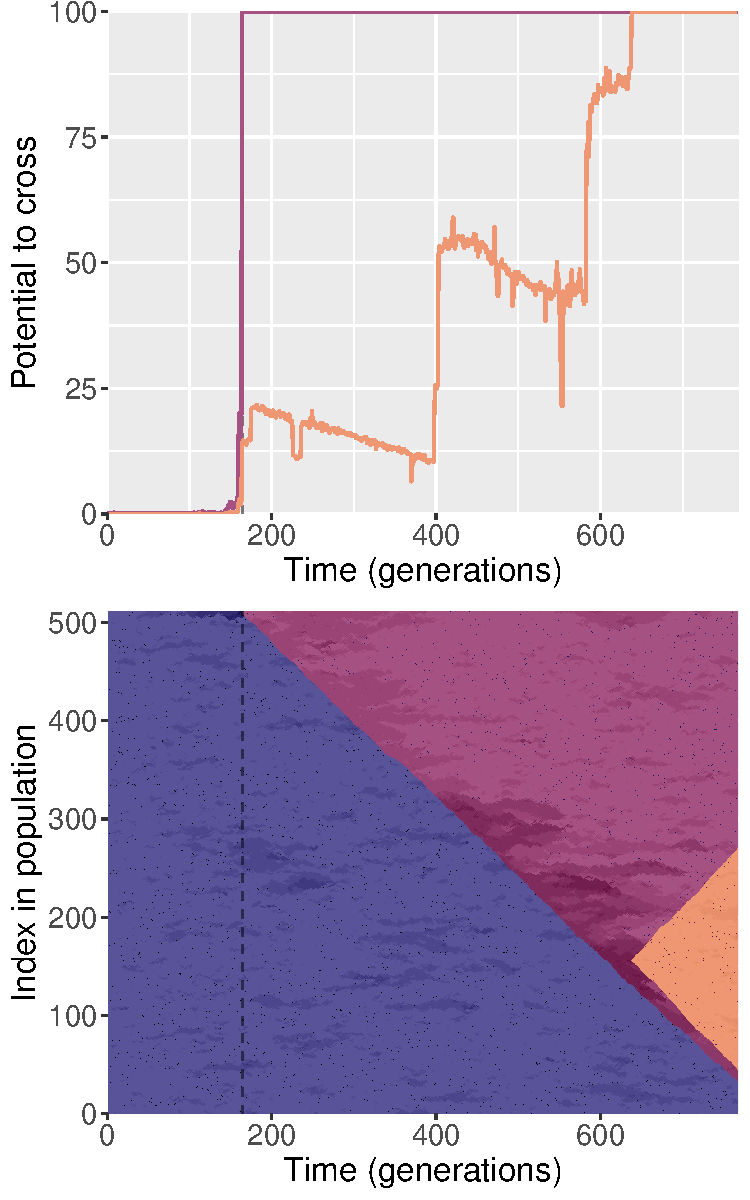
\includegraphics[width=0.6\textwidth]{05_adaptive_momentum/media/reps/no_am_two_cross/script_06__plot_02__combined_plot.pdf}
\caption{
    \textbf{Top plot}: The analytic replay data for the sole replicate that did \textit{not} start in a momentum window, but still managed to cross a valley, and indeed crossed twice. 
    The red line shows the potential to cross the first valley, while the orange line shows the potential to cross the second valley, exhibiting the hallmarks of adaptive momentum due to the first cross. 
    \textbf{Bottom plot}: a Muller plot of the original population, like in Figure \ref{fig-replay-single-cross}.
}
\label{fig-replay-no-window}
\end{center}
\end{figure}

Finally, we also show the potentiation of crossing the second valley, which in some cases is realized (Figs. \ref{fig-replay-double-cross} and \ref{fig-replay-no-window}), and other times is not (Figs. \ref{fig-replay-single-cross} and \ref{fig-replay-no-cross}).
As potentiation is probabilistic in nature, the potential to cross the second valley is the probability of crossing the first valley from the current state of the population times the probability of crossing a second valley from a na\"ive starting position (\textit{i.e.}, the elevated potentiation of a population at the beginning of a sweep). 
We see this dynamic early in the replays -- increases in first-cross potential are reflected, at smaller scales, in second-cross potential,
%Once the first valley is crossed, the potential to cross the second valley can increase dramatically. 
%Indeed, we see sizable increases in second-cross potential 
with a much larger increase upon successful crossing of the first valley in Figures \ref{fig-replay-single-cross} and \ref{fig-replay-double-cross}. %, \ref{fig-replay-no-window}, and . 
This result is consistent with the adaptive momentum framework, which posits that the discovery of a new peak will initiate a new adaptive momentum window. 
Strikingly, this same dynamic holds true for Figure \ref{fig-replay-no-window} -- while the replicate did not start in a momentum window, the first cross creates a window which increases the potential of the second cross.

\subsection{Shuffled population experiments}

To test the importance of population structure for potentiation, we repeated the benchmarking and replay experiments with shuffled populations. 
In both cases, we kept the experiments identical except for an additional shuffle step: before starting a replicate, we shuffled the order of organisms in the population and then proceeded with evolution as normal. 
%We replayed the evolution of 10 randomly-sampled single-cross replicates, and 

The shuffled benchmark data in Figure \ref{fig-combined-plots}C shows that only populations with a leading edge of $p_{2} + 5$ are able to maintain greater than a 10\% chance to cross if the leading edge has swept more than half the population.
Two differences can decrease crossing potential: 
1) multiple leading edges can form, allowing faster fixation and 
2) the eight leading-edge organisms are more likely to encounter higher-fitness mutant-type organisms and thus be purified faster.
%When the benchmark populations are shuffled, fixation occurs more rapidly and thus the potential to cross falls quickly.  

A representative sample from the single-cross replicates is shown in Figure \ref{fig-replay-shuffle}. 
The replay data indicate that potential to cross remains relatively low, never reaching a 20\% chance, until a critical mass of nearly-crossed organisms skyrockets the potential from 9.2\% to 100\%. 
The earlier spikes in potentiation always correspond to the appearance of a single organism that is one step away from crossing the valley, which was then lost in the original population.
These trends are consistent across all 10 replicates that were replayed \citep{austin_ferguson_2024_11507982}. 

\begin{figure}[h!]
\begin{center}
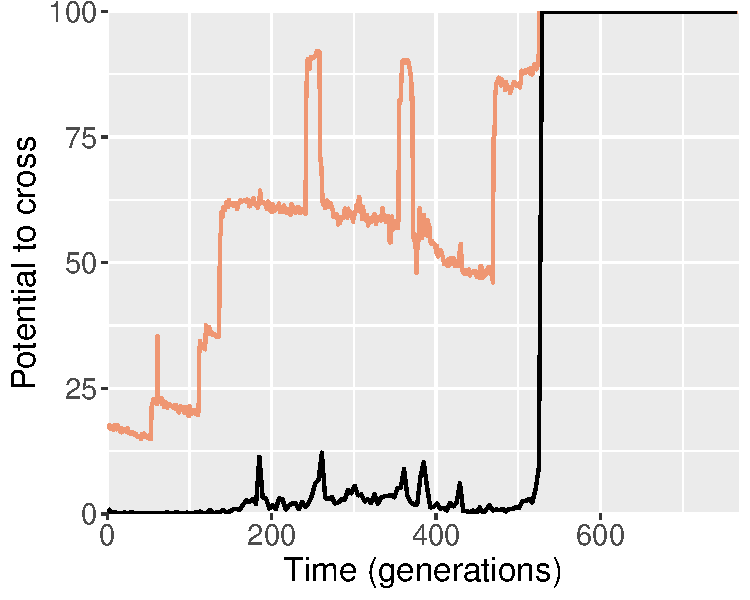
\includegraphics[width=0.6\textwidth]{05_adaptive_momentum/media/reps/400/script_07__plot_01__selected_replays_with_shuffled_replays_no_bg.pdf}
\caption{
    The black line (bottom) shows the potential for a shuffled population to cross a valley. 
    The orange line (top) shows the standard potential for the population to cross (same data as Fig. \ref{fig-replay-single-cross}). 
    The shuffled line consists of 1,000 samples every 4 generations. 
    %Background shading shows the expected potential to cross when an idealized leading edge population is shuffled (a shuffled version of Figure \ref{fig-benchmarking}). 
}
\label{fig-replay-shuffle}
\end{center}
\end{figure}

% \begin{figure}[h!]
% \begin{center}
% 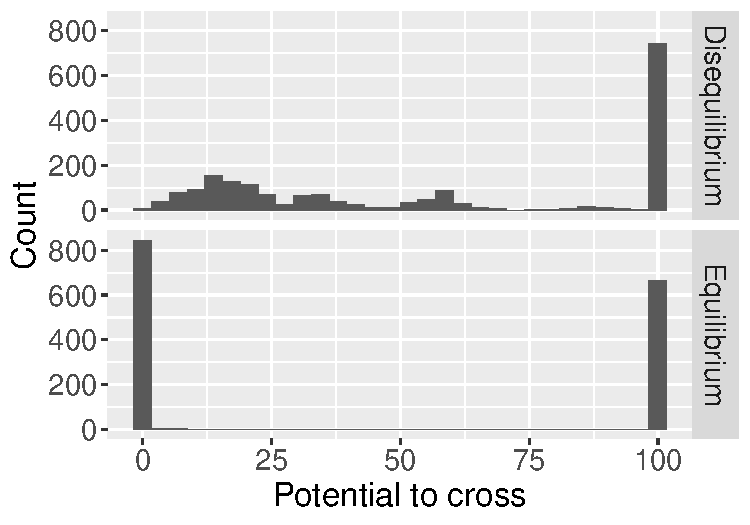
\includegraphics[width=0.45\textwidth]{media/combined_potentiation_histograms.pdf}
% \caption{
%     Histogram of potentiation values in replicates in a momentum window (disequilibrium, top) and outside a window (equilibrium, bottom).
% }
% \label{fig-histograms}
% \end{center}
% \end{figure}









% \section{Results}
% %Below we describe the results in the same order the experiments were described, first validating the adaptive momentum effect, then moving onto benchmarking and replay experiment results.  

% \begin{figure*}[h!]
% \begin{center}
% 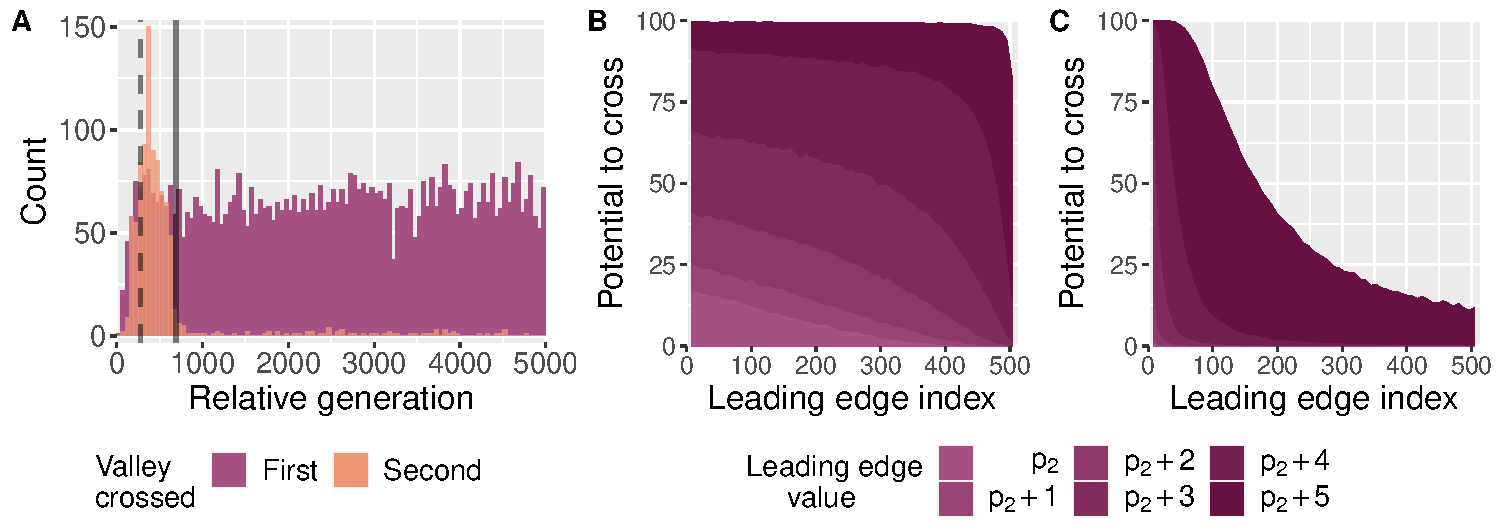
\includegraphics[width=\textwidth]{05_adaptive_momentum/media/combined_plots_full_split.pdf}
% \caption{
%     \textbf{(A)}
%     Distribution of the number of generations required to cross valleys in the validation experiment. 
%     Relative generations refer to the number of elapsed generations for the first cross, and the number of generations since the first cross for the second cross. 
%     %The solid and dashed horizontal lines show the expected count of first and second crosses per bar, respectively, for the expected uniform distribution. 
%     The dashed and solid vertical lines show the minimum and maximum fixation times, respectively. 
%     \textbf{(B)} 
%     Benchmarking data showing the potential of a leading edge to induce a valley cross, with a range of leading edge values and starting positions (see Figure \ref{fig-experiment2}). 
%     Each point represents 10,000 replicates.
%     \textbf{(C)}
%     Shuffled benchmarking data. Each replicate is shuffled prior to evolution, otherwise identical to center plot.
% }
% \label{fig-combined-plots}
% \end{center}
% \end{figure*}

% \subsection{Validation of adaptive momentum effect}

% First, we measured the time it took for replicates starting from a full population of $p_{2}$ to cross valleys.
% Figure \ref{fig-combined-plots}A
% shows the timing distributions of populations that crossed the first valley over the first 5,000 generations (red) as well as the timing distributions of second crossings that occur within 5,000 generations of a first (orange). 
% We see that the time of first crossing appear uniformly distributed across the 5,000 generations, while the second crosses are strongly biased toward shorter time periods. 
% Indeed, of 500,000 replicates, 6,485 crossed the first valley within 5,000 generations (\localapprox 1.3\%) with a mean cross time of \localapprox 2,569 generations and a median of 2,602 generations. 
% Based on these values, we would expect roughly 84 replicates to cross twice ($6,485 \times 1.3\%$, or 0.0169\% of all 500,000 replicates), but instead we see 902 replicates (\localapprox 0.18\%) cross the second valley, showing a much higher rate of second crossing than expected if the probabilities of first and second crossing were equal.
% In addition to a higher than expected rate of crossing, the mean cross time between first and second crossings is \localapprox 579 generations and the median cross time is 401 generations, substantially lower than the first crossing times. 
% Finally, when we consider only those second crossing times that occurred more than 1000 generations after a first crossing, we find that the rate of these second crossings is similar to the first crossing rate (\localapprox 1.23\%).
% These results comport with the framework of adaptive momentum. 
% They show that an initial beneficial discovery can quickly lead to additional discoveries (during the fixation period), but if the second discovery does not happen before equilibrium is reestablished, the rate of valley crossing is better predicted by the first valley crossing times. 


% % Indeed, of 500,000 replicates, 12,793 crossed at least once (\localapprox 2.6\%) with a mean cross time of \localapprox 4,995 generations and a median of 4,951 generations. 
% % We would expect that only 338 replicates to cross twice (2.6\% squared), but instead we see 1,734 replicates cross at least two valleys (\localapprox 0.35\% of total, or \localapprox 13.6\% of those that crossed once). 
% % For the second crossings, we see a mean cross time of 646 generations and a median cross time of 396 generations. 
% % Indeed, while not shown in Figure \ref{fig-crosses-from-scratch}, we see 200 replicates cross at least three valleys, 26 replicates cross at least four valleys, and six replicates cross five valleys; of these higher-order crossings, the median time to cross was always less than 420 generations. 
% % These findings, where an initial beneficial discovery can quickly lead to additional discoveries, supports the initial adaptive momentum theory. 

% % \begin{figure}[h!]
% % \begin{center}
% % 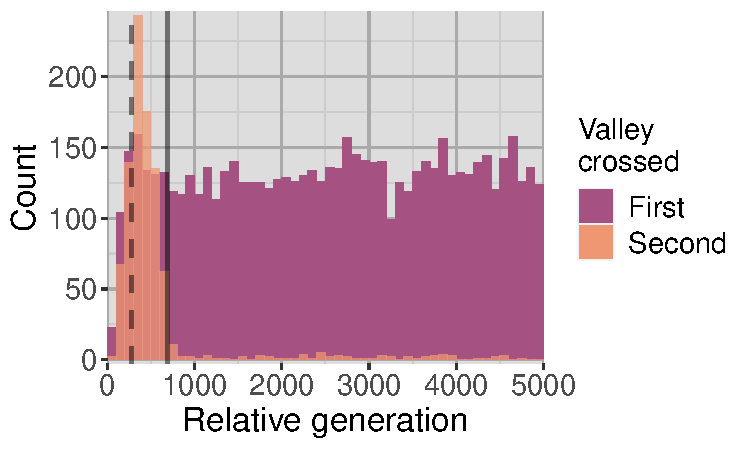
\includegraphics[width=0.45\textwidth]{media/first_two_crosses_overlayed_fair_comparison_with_fixation.pdf}
% % \caption{
% %     Distribution of the number of updates required to cross valleys in the validation experiment. 
% %     Relative updates refer to the number of elapsed generations for the first cross, and the number of generations since the first cross for the second cross. 
% %     %The solid and dashed horizontal lines show the expected count of first and second crosses per bar, respectively, for the expected uniform distribution. 
% %     The dashed and solid vertical lines show the minimum and maximum fixation times, respectively. 
% % }
% % \label{fig-crosses-from-scratch}
% % \end{center}
% % \end{figure}





% %Further, we tested the role of disequilibrium in these discoveries by comparing the evolution of populations seeded with eight organisms on $p_{2}$ and the rest on $p_{1}$ (disequilibrium treatment) against whole populations of $p_{2}$ (control). 
% %We found that 1,751 of 10,000 disequilibrium replicates crossed the first valley (\localapprox 17.5\%), while only 23 of 10,000 control replicates crossed (\localapprox 0.2\%). 
% %This difference is highly significant ($p < 10^{-15}$, Fisher's exact test).
% %This further supports the claim that adaptive momentum relies on disequilibrium in the population, and shows that we can start artificially start an adaptive momentum window in this system by creating this disequilibrium. 

% \subsection{Empirical benchmarks}

% %After confirming that disequilibrium can facilitate valley crosses, we next tested idealized populations to benchmark the effect on valley crossing of two components of this disequilibrium: the position of the leading edge, and the genotypes of the organisms comprising that leading edge.
% The empirical benchmark data (Figure \ref{fig-combined-plots}B) illustrate how the initial state of the population affects the potential to cross valleys.
% %In particular the ratio of the population initiated on $p_2$ (mutant type), versus $p_1$ (wild type) and the value of the individuals on the leading edge,
% As expected, steps further into the valley increase the probability of crossing, regardless of where the leading edge is. 
% On the other hand, the probability of crossing decreases as the ratio of $p_2$ organisms (mutant type) increases relative to $p_1$ organisms (wild type) -- as the selective sweep progresses there are fewer opportunities remaining for additional mutations to accumulate. 
% While the potential to cross varies considerably with the type of organisms in the leading edge, these data clearly show that all conditions describing early sweep conditions (i.e., having leading edge and a significant ratio of the remaining population on $p_1$) %having any leading edge 
% substantially increase the probability of crossing the valley compared to populations that are close to reaching equilibrium on $p_2$. 

% %The benchmarks with a leading edge at index 0 see slightly lower rates of crossing, as they only have one organism at the given value while every other point has 8 organ
% %We typically ran these benchmarking populations with a leading edge of eight organisms of the same type to remove the possibility of genetic drift immediately destroying the leading edge. 
% %This drift accounts for the drop in crosses at index 0, the one instance where the leading edge consisted of only a single organism. 
% %Finally, being one step away from crossing the valley ($p_2$ + 5) effectively guarantees a cross, as eight organisms at that value are almost certain to accumulate the one needed mutation unless the selective sweep is almost over. 
% %Overall, these data match our expectations. 
% We use these results to provide a baseline prediction for the analytic replay experiments. 

% % \begin{figure}[h!]
% % \begin{center}
% % 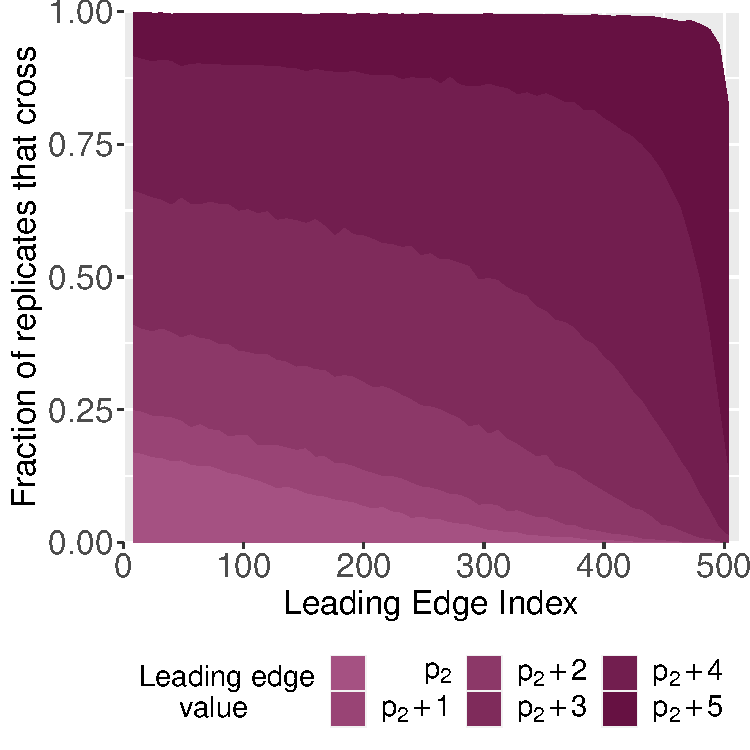
\includegraphics[width=0.45\textwidth]{media/benchmarking_area.pdf}
% % \caption{
% %     Benchmarking data showing the potential of a leading edge to induce a valley cross, with a range of leading edge values and starting positions. 
% %     The leading edge always consists of eight organisms of that value. 
% %     Each point represents 10,000 replicates. 
% % }
% % \label{fig-benchmarking}
% % \end{center}
% % \end{figure}

% \subsection{Analytic replay experiments}
% Of our 500 initial replicates to find candidates for replay experiments, four replicates (0.8\%) crossed two valleys in the allotted time, 83 crossed exactly one valley (16.6\%), and the remaining 413 did not cross any valleys (82.6\%). 
% We ran coarse-grained replays for 10 randomly-sampled no-cross replicates, 10 random single-cross replicates, and all four double-cross replicates.
% %We ran coarse-grained analytic replay experiments for all four replicates that crossed twice and for 10 randomly-sampled replicates of each of the two other categories. 
% %For each of these 24 replicates, we replayed at every fourth generation, with 1,000 replicates per time point. 
% All plots are available in the supplement \citep{austin_ferguson_2024_11507982}. 

% From these coarse-grained replays, we selected one representative replicate from each category. 
% We re-ran these representative replicates, conducting 10,000 replay trials at \textit{every} time point to give a fine-grained view. 
% %We show the replay results in two formats. 
% %The first showing the potential of crossing the next valley over time and the second as Muller plots showing the underlying population structure that beget that potentiation. 
% For each replayed replicate, we show the potential of crossing the next valley over time, paired with a Muller plot \citep{mullerGeneticAspectsSex1932} of the initial replicate that was replayed. 
% Figures \ref{fig-replay-single-cross}, \ref{fig-replay-double-cross}, and \ref{fig-replay-no-cross} show the single-cross, double-cross, and no-cross replicates, respectively. 
% %In each plot, the replay results are overlaid atop the benchmarking data, which has been adjusted such that the leading edge index aligns with the actual leading edge at that generation of the population.
% In each plot, the replay results are overlaid atop an image generated from the benchmark data. 
% %To generate the background image, we treat the benchmark data as a lookup function and use the current position of the leading edge of the replay result to look up the potentiation predicted by the benchmark data. 
% To generate the background image, we treat the benchmark data as a lookup function. 
% When we start a replay replicate, we initialize the population using the snapshot from a particular generation of the initial replicate. 
% These snapshots show that the leading edge does not perfectly advance one position every generation; there are many generations where the leading edge either fails to advance or is pushed back one position by the wild type organisms.
% %As we see in our population snapshots, the leading edge does not actually advance one position every generation, the leading often fails to advance, and occasionally the wild-type organisms replicate over the leading edge, pushing it back one step. 
% To make this comparison fair, we find the leading edge in that particular snapshot and then look up the corresponding expectation values from the benchmark data. 
% %Thus, the background image shows in ``real time'' potentiation of the replay at each generation.
% This adjustment ensures that we are comparing against the correct benchmark data regardless of the motion of the leading edge. 
% %Thus, the background image adjusts 

% Overall, the potentiation observed in all three replicates closely match the benchmark expectations. 
% The potentiation occasionally increases or decreases suddenly; tracing these changes to the Muller plots typically shows that these events correlate to the gain or loss of a mutation at (or near) the leading edge at that time. 
% For example, the two temporary peaks in potential in Figure \ref{fig-replay-single-cross}, at roughly generations 250 and 375, can be directly traced to the leading edge temporarily dipping to $p_{2} + 4$.
% %When the leading edge mutates further into the fitness valley, the potentiation increases dramatically. 
% %Each of the three replicates 
% The potentiation at any particular step in the valley decreases over time, as the selective sweep progresses and the adaptive momentum window closes.
% Figure \ref{fig-replay-no-cross} clearly shows that, while the replicate had substantial potentiation at times (briefly above 50\%), it failed to capitalize before the window closed. 
% This failure was exacerbated by two leading mutations from $p_{2} + 3$ to $p_{2} + 2$, the second of which dropped the potential from over 25\% to under 10\%, after which the population never recovers. 
% % It should be noted that the dramatic increases or decreases in potentiation can be mapped cleanly onto the Muller plots showing the state of the population. 
% % For example, in Figure \ref{fig-replay-single-cross} potentiation temporarily increases dramatically (from \localapprox 60\% to \localapprox 90\%) twice, once around update 250 and again around update 350. 
% % In both cases, the potentiation then drops to previous levels shortly after. 
% % Mapping this points onto the Muller plot, we see that, in both cases, the leading edge drifted down an additional step into the valley (to $p_{1} + 4$) before quickly drifting back to the previous step. 
% % These drops in potentiation are particularly dramatic in the no-cross replicate of Figure \ref{fig-replay-no-cross}, where a late drift backward reduces the potential to cross from over 25\% to under 10\%, from which the population never recovers. 

% All three replicates show periods of potentiation higher than what our benchmark data would predict given their leading edge genomic value. 
% The benchmarking data modeled a leading edge of eight organisms, but the Muller plots show that the leading edge grows and shrinks over time. 
% The Muller plots show that overprediction is generally associated with either an expanded leading edge or an excess of individuals with lower fitness behind the leading edge. 
% We hypothesized that these overpredictions are generally observed in deeper steps into the valley because of the historical contingency required to reach that point (i.e., to reach $p_{2} + 5$ the leading edge must have passed through $p_{2} + 4$, which may still exist behind the leading edge).
% %While all organisms behind the leading edge are experiencing purifying selection, this purification takes time, and a cluster of mutated organisms can persist behind the leading edge. 
% %Our benchmark expectations are particularly accurate for early steps into the valley; even if a large cluster of organisms exists behind the leading edge, they are still unlikely to accumulate the needed mutations to cross the valley before being purified. 
% %In contrast, when the leading edge is only a mutation or two away from crossing, even a few organisms trailing the leading edge can be enough to cross the valley. 
% %If a sizable section of the population is only two or three mutations from crossing the valley, the size of that section may buffer the organisms from purifying selection long enough for some organisms to genetically drift to the next peak. 
% %This is supported by the replays almost perfectly aligning with the expectation in the first few steps into the valley, where the mutation rate cannot outpace the rate of purifying selection, while the empirical potentiation is often above the expectation in the last few steps of the valley. 
% %This was not explicitly modeled in the benchmarking data, possibly causing this difference. 
% %while replays see leading edges that are much larger or smaller, causing some variation from the expectation.
% %Further, our benchmarks are based \textit{only} on the leading edge, and thus our hypothesis is that this higher-than-expected potentiation results from the evolutionary potential of non-leading edge organisms. 

% \begin{figure}[h!]
% \begin{center}
% 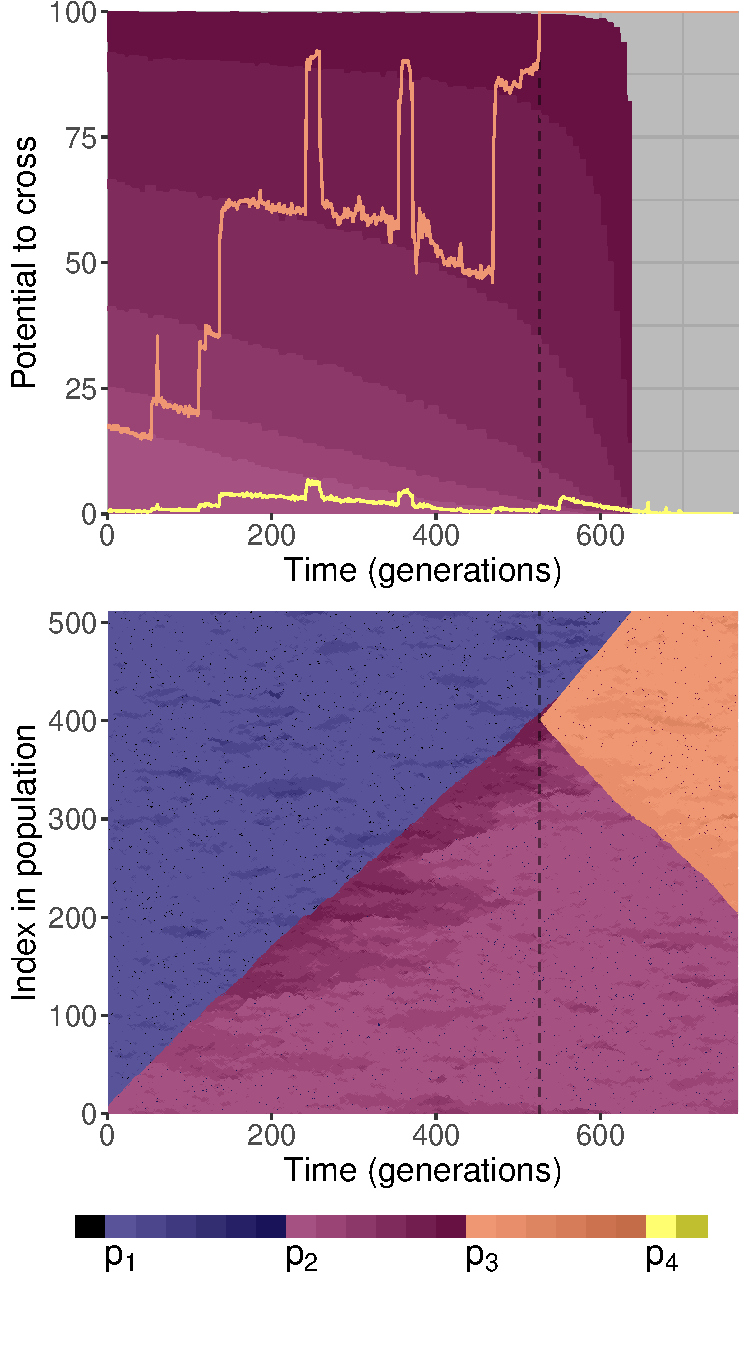
\includegraphics[width=0.6\textwidth]{05_adaptive_momentum/media/reps/400/script_06__plot_05__combined_plot_area_palette.pdf}
% \caption{
%     \textbf{Top plot}: The analytic replay data for a representative replicate that crossed one valley during a momentum window. 
%     The two lines show the probability of crossing valleys, with the initially-higher (orange) line showing the first valley cross and the initially-lower (yellow) line showing the second valley cross. 
%     The background shading shows the expected potential to cross (as shown in Figure \ref{fig-combined-plots}B), adjusted by the actual leading edge of the population. 
%     Each update was replayed 10,000 times. 
%     \textbf{Bottom plot}: A Muller plot of the original population over time. 
%     Dark colors show descent into a valley, with hue identifying the valley being crossed. 
%     In both plots, vertical lines show valley crosses.
%     Colors in the legend apply to all plots. 
% }
% \label{fig-replay-single-cross}
% \end{center}
% \end{figure}

% \begin{figure}[h!]
% \begin{center}
% 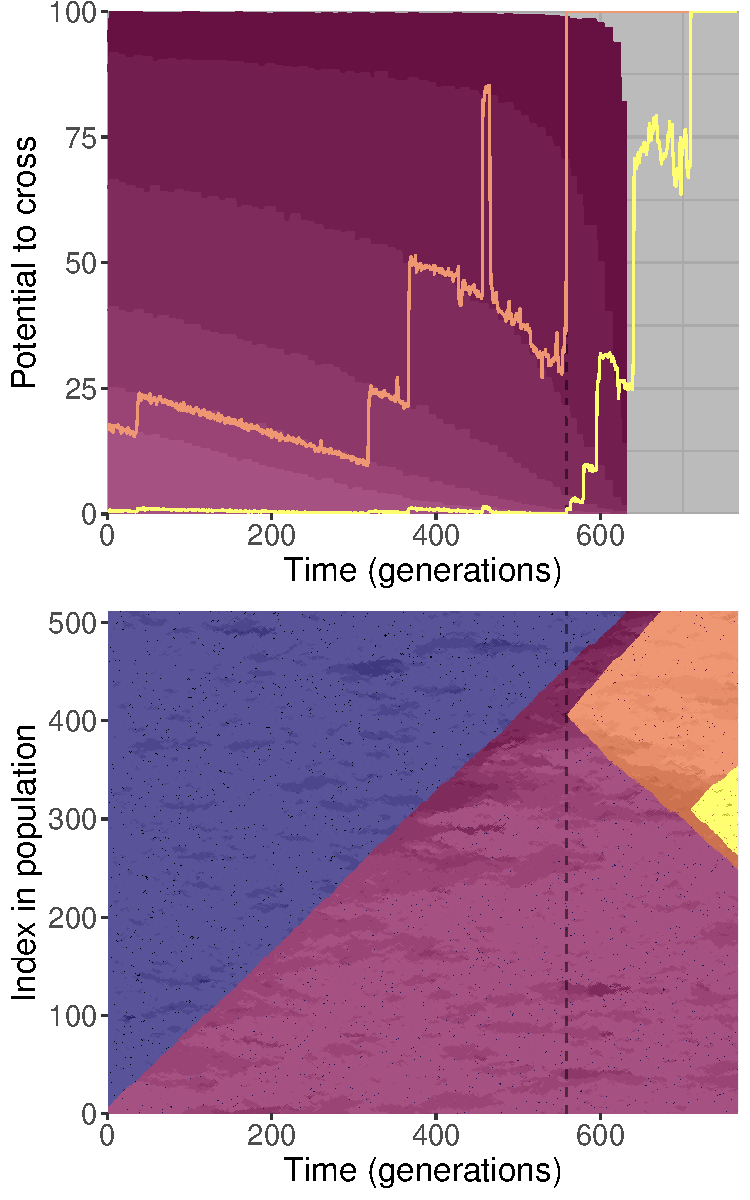
\includegraphics[width=0.6\textwidth]{05_adaptive_momentum/media/reps/263/script_06__plot_03__combined_plot_area.pdf}
% \caption{
%     The analytic replay data for a representative replicate that crossed two valleys during a momentum window. 
%     See Figure \ref{fig-replay-single-cross} for details and legend. 
% }
% \label{fig-replay-double-cross}
% \end{center}
% \end{figure}

% \begin{figure}[h!]
% \begin{center}
% 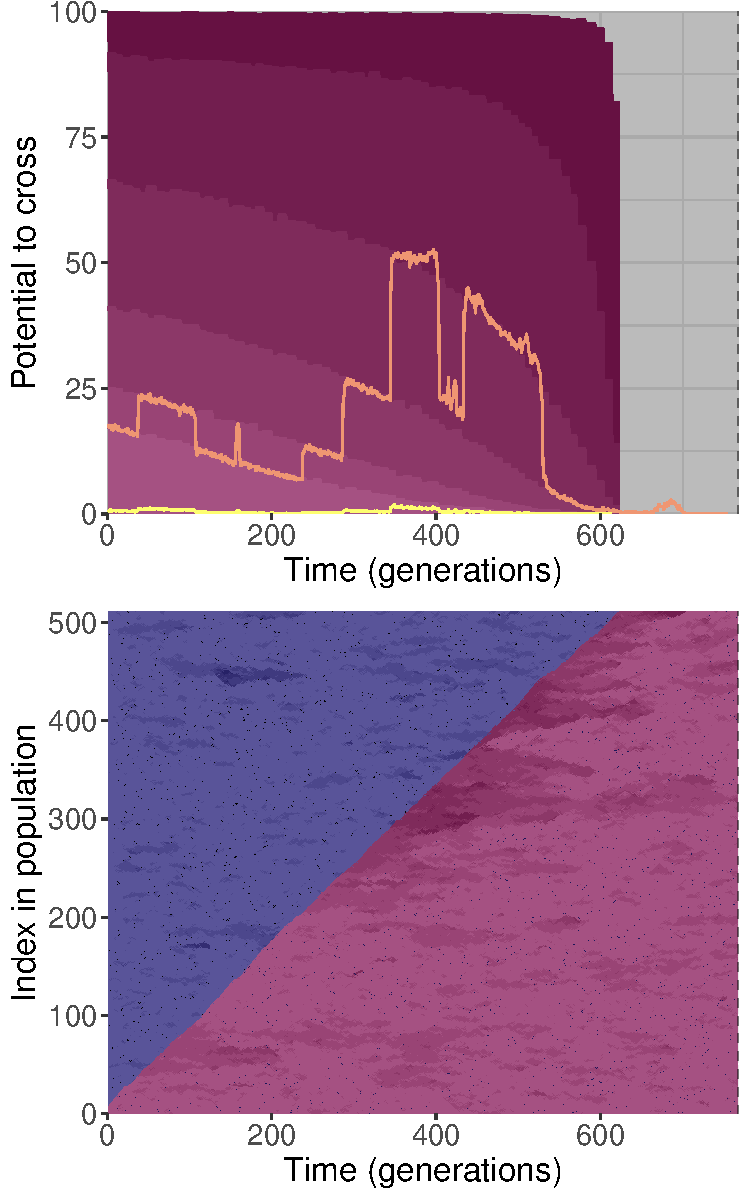
\includegraphics[width=0.6\textwidth]{05_adaptive_momentum/media/reps/339/script_06__plot_03__combined_plot_area.pdf}
% \caption{
%     The analytic replay data for a representative replicate that failed to cross a valley during a momentum window.
%     See Figure \ref{fig-replay-single-cross} for details and legend.
% }
% \label{fig-replay-no-cross}
% \end{center}
% \end{figure}

% For comparison, we also replayed replicates that did not start in a momentum window. 
% We replayed the one replicate in 10,000 that crossed twice, 10 randomly sampled replicates that crossed once, and 10 random replicates that failed to cross. 
% Figure \ref{fig-replay-no-window} shows the replicate that crossed twice. 
% The first crossing in this replicate occurred quite early, crossing the valley on generation 168. 
% However, the potential before crossing is similar to all first-cross replicates: while the potential in an adaptive momentum window starts at \localapprox 17\%, the potential for replicates outside momentum windows starts at \localapprox 0.2\%. 
% This low potential continues for the first 143 generations, followed by 16 generations with an average potential of \localapprox 1.8\%, four generations between 15\% and 20\%, and then the cross. 
% %This pure chance, ``all or nothing'' potentiation is not unique to this replicate, as we see in the histograms of potential shown in Figure \ref{fig-histograms}.
% This pure chance, ``all or nothing'' potentiation is not unique to this replicate; the same dynamic can be seen in the ten other succesful replicates we analyzed \citep{austin_ferguson_2024_11507982}.
% % Figure \ref{fig-replay-no-window} shows the potential for the first and second valley crossing. 
% % The potential for the first valley crossing remains very low ($<$0.4\%) until it increased to 100\% in less than 20 generations. 
% % This increase is not linear, however, as there is an initial increase and then a drop in potentiation, likely corresponding to the flux in $p_{2} + 5$ organisms in the population. 
% % The discovery of $p_{3}$ starts a momentum window, and the potential of the second cross then looks like the potential in previous results (although limited by the lack of remaining time), and is higher than the potential of the first window was for the first \localapprox 580 generations.


% \begin{figure}[h!]
% \begin{center}
% 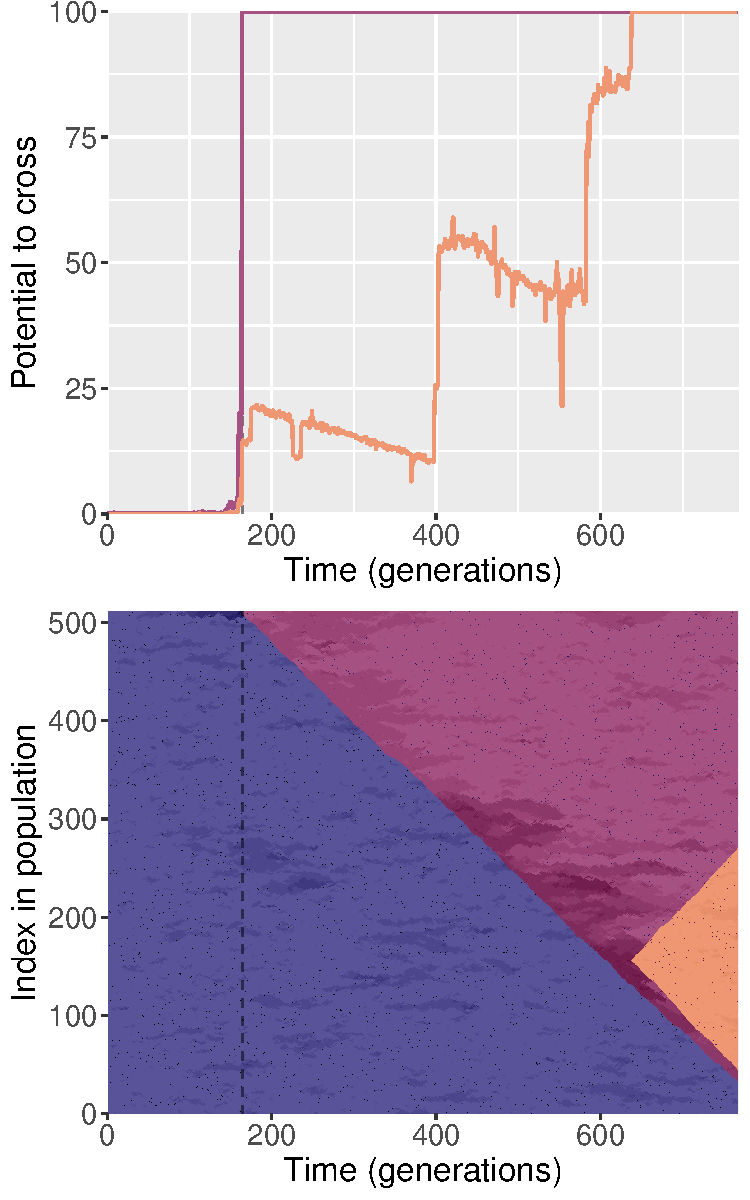
\includegraphics[width=0.6\textwidth]{05_adaptive_momentum/media/reps/no_am_two_cross/script_06__plot_02__combined_plot.pdf}
% \caption{
%     \textbf{Top plot}: The analytic replay data for a representative replicate that did \textit{not} start in a momentum window but still managed to cross a valley. 
%     The red line shows the potential to cross the first valley, while the orange line shows the potential to cross the second valley. 
%     \textbf{Bottom plot}: a Muller plot of the original population, like in Figure \ref{fig-replay-single-cross}.
% }
% \label{fig-replay-no-window}
% \end{center}
% \end{figure}

% Finally, we also show the potentiation of crossing the second valley, which in some cases is realized (as in Figures \ref{fig-replay-double-cross} and \ref{fig-replay-no-window}), and other times is not (Figures \ref{fig-replay-single-cross} and \ref{fig-replay-no-cross}).
% As potentiation is probabilistic in nature, the potential to cross the second valley can be thought of as the product of crossing the first valley from the current state of the population and the probability of crossing a second valley from a naive starting position (i.e, the elevated potentiation of a population at the beginning of a sweep). 
% We see this dynamic reflected early in the replays -- increases in first-cross potential are reflected, at much smaller scales, in second-cross potential. 
% Once the first valley is crossed, the potential to cross the second valley can increase dramatically. 
% We see sizable increases in second-cross potential upon successful crossing of the first valley in Figures \ref{fig-replay-single-cross} and \ref{fig-replay-double-cross}. %, \ref{fig-replay-no-window}, and . 
% This result is consistent with adaptive momentum framework, which posits that the discovery of a new peak will initiate a new adaptive momentum window. 
% Most strikingly, this same dynamic holds true for Figure \ref{fig-replay-no-window} -- while the replicate did not start in a momentum window, we see the first cross create a window and the potential of the second cross reflects that.

% \subsection{Shuffled population experiments}

% To test the effect of population structure on potentiation, we repeated the benchmarking and replay experiments with shuffled populations. 
% In both cases, the experiments were repeated exactly, except for one additional shuffle step: before beginning to evolve the populations, we would shuffle the order of organisms in the population, and then proceed with evolution as normal. 
% %We replayed the evolution of 10 randomly-sampled single-cross replicates, and 

% The shuffled benchmark data in Figure \ref{fig-combined-plots}C shows that only populations with a leading edge of $p_{2} + 5$ are able to maintain greater than a 10\% chance to cross if the leading edge has swept more than half the population.
% Two differences arise when we shuffle the benchmark populations that can decrease crossing potential: 
% 1) fixation can occur faster because of multiple leading edges and 
% 2) when the eight organisms from the leading edge are shuffled into the population, they are likely to be purified faster.
% %When the benchmark populations are shuffled, fixation occurs more rapidly and thus the potential to cross falls quickly.  

% A representative sample from the 10 single-cross replicates is shown in Figure \ref{fig-replay-shuffle}. 
% The replay data indicate that potential to cross remains relatively low, never reaching a 20\% chance, until a critical mass of nearly-crossed organisms skyrockets the potential from 9.2\% to 100\%. 
% The earlier spikes in potentiation always correspond to the appearance of a single organism that is one step away from crossing the valley, which was then lost in the original population.
% These trends were consistent across all 10 replicates that were replayed \citep{austin_ferguson_2024_11507982}. 

% \begin{figure}[h!]
% \begin{center}
% 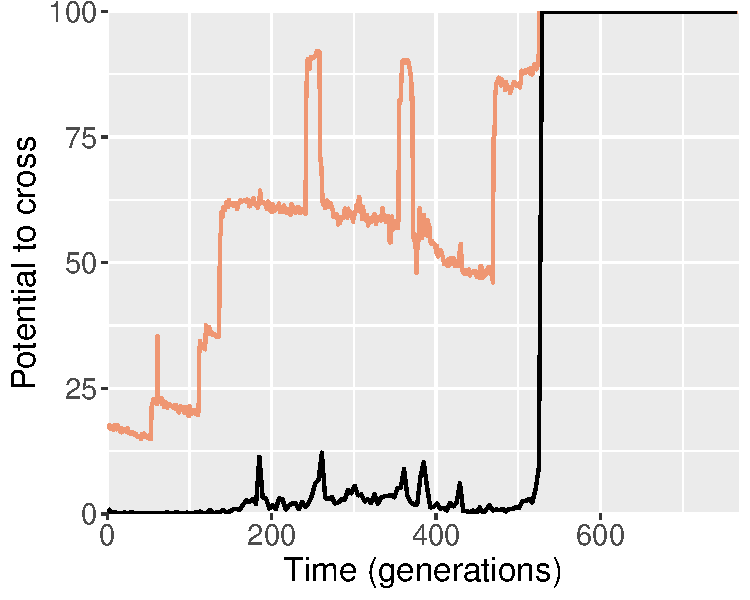
\includegraphics[width=0.6\textwidth]{05_adaptive_momentum/media/reps/400/script_07__plot_01__selected_replays_with_shuffled_replays_no_bg.pdf}
% \caption{
%     The black line (bottom) shows the potential for a shuffled population to cross a valley. 
%     The orange line (top) shows the standard potential for the population to cross (same data as Figure \ref{fig-replay-single-cross}). 
%     The shuffled line consists of 1,000 samples every 4 generations. 
%     %Background shading shows the expected potential to cross when an idealized leading edge population is shuffled (a shuffled version of Figure \ref{fig-benchmarking}). 
% }
% \label{fig-replay-shuffle}
% \end{center}
% \end{figure}

% % \begin{figure}[h!]
% % \begin{center}
% % 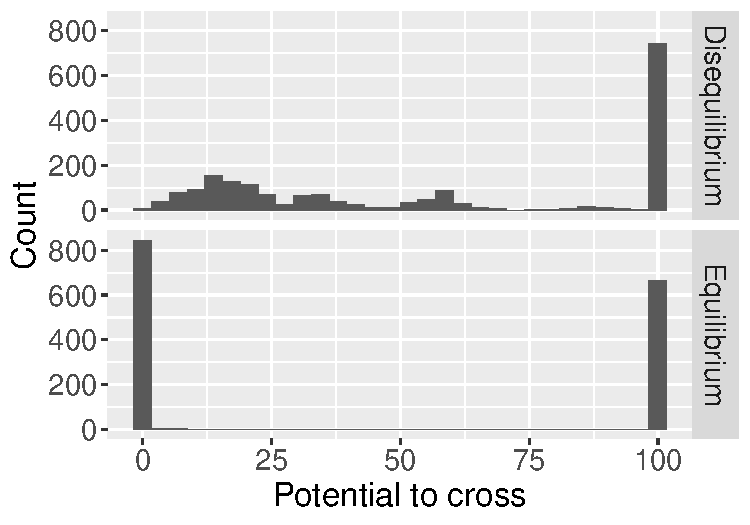
\includegraphics[width=0.45\textwidth]{media/combined_potentiation_histograms.pdf}
% % \caption{
% %     Histogram of potentiation values in replicates in a momentum window (disequilibrium, top) and outside a window (equilibrium, bottom).
% % }
% % \label{fig-histograms}
% % \end{center}
% % \end{figure}


\section{Discussion and Conclusion}

% Crossing is pure chance without AM
%   But has some baseline probability under AM
%\subsection{Adaptive momentum can drastically alter a population's potential}
\subsection{Potentiation exhibits adaptive momentum}

In this work, we have corroborated adaptive momentum's benefit to valley crossing (as outlined in \citep{Bohm2024.04.08.588357}) and expanded our understanding of the dynamic. 
Our initial experiments demonstrated that our system can undergo adaptive momentum, and that disequilibrium is the key driver. 
However, our main goal in this paper is to provide an alternate vantage point from which to view the dynamics of adaptive momentum. 
While the original paper validated the effect via aggregated data, here we analyze the underlying dynamics in action on individual populations by quantifying potentiation via replay experiments. 

We have shown that populations outside of momentum windows must rely on chance alone to cross a valley. 
During these ``equilibrium'' periods, early mutations into the valley, although required for a valley crossing, have no substantial impact on the population's probability of crossing. 
Conversely, populations in momentum windows immediately see a drastically higher chance to cross, and every mutation in the leading edge is either potentiating or anti-potentiating, depending on the direction. 
This result is highlighted in Figure \ref{fig-replay-no-window}, where the first cross was pure chance while the second cross was driven by adaptive momentum.
This work is only a beginning; future work should apply these techniques to examine the role of adaptive momentum in more complex and realistic fitness landscapes.

% Do we need something to tie this section together


% The leading edge value almost perfectly predicts potentiation for the first few steps
\subsection{The leading edge in a spatial selective sweep determines potentiation}
%\subsection{The position and state of the leading edge of a selective sweep determines its adaptive potential}

The adaptive momentum framework posits that disequilibrium in a population can reduce the selection pressure on the advantaged subpopulation \citep{Bohm2024.04.08.588357}.
In spatial populations, disequilibrium is focused at the leading edge of selective sweeps, where advantaged mutants encroach on the wild type. %, which is exactly what we see here. 
Indeed, we observe that the genotype of the organism at the leading edge of the sweep is a strong predictor of potentiation. 
Moreover, as we can see in the Muller plots, there are often mutated organisms lagging the leading edge. 
When the leading edge is further into the valley, those lagging organisms have a non-negligible chance to accumulate sufficient mutations to finish crossing the valley, thus increasing the potential.

We aimed to create the simplest system for studying valley crossing in spatial populations.
In these one-dimensional populations, our artificially-started sweeps have exactly one leading edge. % (although self-actuated sweeps may have two or more). 
These edges become more complex in two-dimensional digital systems and only increase in complexity moving toward more natural systems. 
While the identification and measurements of the leading edge may become more difficult, we expect similar dynamics to hold. 
It is critical that we continue to improve our understanding of adaptive momentum in these simple systems to build a solid theoretical foundation. 
%We expect that similar dynamics will unfurl in these more complicated systems, but with many more intricacies. 
%For example, here our potential to cross in a momentum window moves in predictable and sizable steps because we have only one organism at the leading edge. 
%In more complex systems, these dynamics will be much harder to identify. 


% When we take population snapshots, potentiation looks great
%   If we shuffle the population, potentiation is very low until we cross
%   If we do clonal restarts, potentiation is only ever ~0% and ~100%
\subsection{Population heterogeneity and structure affect potentiation}

Previous experiments have conducted analytic replays starting from clonal populations \citep{blountHistoricalContingencyEvolution2008, fergusonPotentiatingMutationsFacilitate2023}. 
Here, however, we used perfect population snapshots that record every organism in every generation. 
Our technique provides a more fine-grained look into how potentiation changes. 
%In fact, if we had started with clonal populations of the most abundant genotype as in previous work, we would only see a maximum of four clones per replicate ($p_{1}$, $p_{2}$, $p_{3}$, and $p_{4}$) because at no time during any of our experiments is the dominant type in a population not a purebred type.
Furthermore, previous work has often used the most abundant genotype at a time point to seed replay experiments. 
Across all of our experiments, the most abundant genotype was always on one of the peaks. % ($p_{1}$, $p_{2}$, $p_{3}$, or $p_{4}$).
Replays looking at the potential of the first cross would see effectively zero probability for $p_{1}$ and $p_{2}$ and 100\% probability for $p_{3}$ and $p_{4}$, which have already crossed, missing all nuance and change in this potential. 

The nuance gained by replaying population snapshots provides important insight into using analytic replay experiments, and puts the large jumps in potentiation seen in previous work into question \citep{fergusonPotentiatingMutationsFacilitate2023}.
While those large jumps in potentiation are valid, they are likely missing important intermediate genotypes or population dynamics. 
In effect, they show genetic effects isolated from effects of population structure.
%Future work should use population snapshots when possible, and further analysis into the effect of using population snapshots instead of clonal restarts should be further disentangled in simple models like this one. 
Future work looking to leverage replay experiments should be aware that population structure and composition can affect evolutionary outcomes, and should thus carefully consider how replays are initialized. 
%This work signifies the first step in using genetic potentiation to study population dynamics. 

Further, by shuffling the population snapshots we have shown that it is not just the portion of the population with each genotype that matters, but also the structural relationships and interactions among the organisms (Figure \ref{fig-replay-shuffle}).
Other computational studies will likely be needed to tease apart when and how this organization matters %; however, while replay experiments of natural organisms are always monumental amounts of work, 
as perfectly preserving structure and composition of natural populations for so many replicates is currently impossible. 
As such, we should leverage computational models to develop techniques possible in both digital and natural populations, possibly finding a middle ground between a single clonal sample and full population snapshots. 
%The organization of the population matters in two ways: 1) preservation of the leading edge and 2) formation of ``depressed'' region. 
%When we shuffle a population, the leading edge might have fewer organisms left to sweep and thus fewer opportunities for mutations, or, worse, be isolated to only a few organisms that are then purged by purifying selection or genetic drift. 
%As we see in Figure \ref{fig-replay-double-cross}, valley crosses sometimes occur slightly behind the leading edge in a mutated region that has not yet been subjected to purifying selection. 
%In these cases, the size of the region matters -- the more organisms in it the longer it will take for them all to be purified. 
%We have shown that when we shuffle the population, we are destroying these regions and thus limiting potential to cross. 

\subsection{Outlook}


%This work not only serves to replicate the expectations of adaptive momentum, but effectively exposes the underlying mechanisms. 
%By quantifying potentiating and relating this to population composition and structure, we have strengthened the arguments proposed by adaptive momentum theory while also expanding the use cases for potentiation and replay experiments as analytical tools.

This work not only provides evidence to support our understanding of adaptive momentum, but further clarifies the underlying mechanisms. 
By quantifying the potentiation of valley crosses and relating this measure to population composition and structure, we have % strengthened the arguments proposed in the adaptive momentum framework and 
provided insights into the historical contingencies and long-term trajectories of populations experiencing adaptive momentum. 
Further, we advance the methodology of analytic replay experiments by conducting them at a greater scale than previously seen, demonstrating a new use case, and leveraging perfect population snapshots to seed the replay experiments. 
These advances combine to show that replay experiments can extend genetic potentiation to include the effects of population dynamics. 
All together, this work constitutes both a step toward better understanding adaptive momentum and a methodological refinement of replay experiments for understanding historical contingency.












% \section{Discussion and Conclusion}

% % Crossing is pure chance without AM
% %   But has some baseline probability under AM
% %\subsection{Adaptive momentum can drastically alter a population's potential}
% \subsection{Potentiation exhibits adaptive momentum}

% In this work, we have corroborated adaptive momentum's benefit to valley crossing originally outlined in \citep{Bohm2024.04.08.588357}. 
% Our initial experiments demonstrated that our system can experience adaptive momentum, and that disequilibrium is the key driver. 
% However, the main goal of this paper is to provide an alternative vantage point from which to view the dynamics of adaptive momentum. 
% While the original paper validated the effect via aggregated data, here we analyze the underlying dynamics in action on individual populations by quantifying potentiation via replay experiments. 

% We have shown that populations outside of momentum windows must rely on chance alone to cross the valley. 
% During these ``equilibrium'' periods, early mutations into the valley, although required for a valley crossing, have no substantial impact on the population's probability of crossing. 
% Conversely, populations in momentum windows immediately see a drastically higher chance to cross, and every mutation in the leading edge is either potentiating or anti-potentiating, depending on the direction. 
% This is highlighted in Figure \ref{fig-replay-no-window}, where the first cross was pure chance while the second cross was driven by adaptive momentum.
% This work is only the beginning, and future work should apply similar techniques to understanding the role of adaptive momentum in other, more complex, fitness landscapes.

% % Do we need something to tie this section together


% % The leading edge value almost perfectly predicts potentiation for the first few steps
% \subsection{The leading edge in a spatial selective sweep determines potentiation}
% %\subsection{The position and state of the leading edge of a selective sweep determines its adaptive potential}

% The adaptive momentum framework posits that disequilibrium in a population can reduce the selection pressure on the advantaged subpopulation \citep{Bohm2024.04.08.588357}.
% In a spatial populations, disequilibrium is focused at the leading edge of selective sweeps, where the advantaged mutants will continue to encroach on the wild type. %, which is exactly what we see here. 
% Indeed, we observe that the genotype of the organism at the leading edge of the sweep is a strong predictor of potentiation in this system. 
% Moreover, as we can see in the Muller plots, there is often a cluster of mutated organisms lagging the leading edge. 
% When the leading edge is further into the valley and fewer mutations are needed to cross, those lagging organisms have a non-negligible chance to accumulate sufficient mutations and cross the valley, increasing the potential.

% We aimed to create the simplest system for studying the leading edge of spatial populations.
% In these one-dimensional populations, our artificially-started sweeps have exactly one leading edge. % (although self-actuated sweeps may have two or more). 
% These edges become more complex in two-dimensional digital systems and only increase in complexity moving toward more natural systems. 
% While the identification and use of the leading edge for making predictions may become more difficult, we expect similar dynamics to hold. 
% It is critical that we continue to improve our understanding of adaptive momentum in these simple systems to build a solid foundation to expand upon. 
% %We expect that similar dynamics will unfurl in these more complicated systems, but with many more intricacies. 
% %For example, here our potential to cross in a momentum window moves in predictable and sizable steps because we have only one organism at the leading edge. 
% %In more complex systems, these dynamics will be much harder to identify. 


% % When we take population snapshots, potentiation looks great
% %   If we shuffle the population, potentiation is very low until we cross
% %   If we do clonal restarts, potentiation is only ever ~0% and ~100%
% \subsection{Population heterogeneity and structure affect potentiation}

% Previous work using analytic replay experiments have started the replays with clonal populations \citep{blountHistoricalContingencyEvolution2008, fergusonPotentiatingMutationsFacilitate2023}. 
% Here, however, we ran replays with perfect population snapshots that record every organism in every generation. 
% This technique provides a more fine-grained look into how potentiation changes. 
% %In fact, if we had started with clonal populations of the most abundant genotype as in previous work, we would only see a maximum of four clones per replicate ($p_{1}$, $p_{2}$, $p_{3}$, and $p_{4}$) because at no time during any of our experiments is the dominant type in a population not a purebred type.
% Previous work has used the most abundant organism at a time point to seed replay experiments. 
% Across all of our experiments, the most abundant organism type was always on one of the peaks. % ($p_{1}$, $p_{2}$, $p_{3}$, or $p_{4}$).
% Replays looking at the potential of the first cross would see effectively zero probability for $p_{1}$ and $p_{2}$ and 100\% probability for $p_{3}$ and $p_{4}$, which have already crossed, missing all nuance and change in this potential. 

% The nuance gained by replaying population snapshots provides important insight into using analytic replay experiments, and puts the large jumps in potentiation seen in previous work into question \citep{fergusonPotentiatingMutationsFacilitate2023}.
% While those large jumps in potentiation are valid, they are likely missing important intermediate genotypes or population dynamics. 
% In effect, they show genetic effects isolated from effects of population structure.
% %Future work should use population snapshots when possible, and further analysis into the effect of using population snapshots instead of clonal restarts should be further disentangled in simple models like this one. 
% Future work looking to leverage replay experiments should be aware of the effect that population structure and composition can have on evolutionary outcomes, and should thus carefully consider how replays are initialized. 
% %This work signifies the first step in using genetic potentiation to study population dynamics. 

% Further, by shuffling the population snapshots we have shown that it is not just the portion of the population with each genotype that matters, but also the structural relationships and interactions among the organisms (Figure \ref{fig-replay-shuffle}).
% Other computational studies will likely be needed to tease apart when and how this organization matters %; however, while replay experiments of natural organisms are always monumental amounts of work, 
% as perfectly preserving structure and composition of natural populations for so many replicates is currently impossible. 
% As such, we should leverage computational models to develop techniques possible in both digital and natural populations, possibly finding a middle ground between a single clonal sample and full population snapshots. 
% %The organization of the population matters in two ways: 1) preservation of the leading edge and 2) formation of ``depressed'' region. 
% %When we shuffle a population, the leading edge might have fewer organisms left to sweep and thus fewer opportunities for mutations, or, worse, be isolated to only a few organisms that are then purged by purifying selection or genetic drift. 
% %As we see in Figure \ref{fig-replay-double-cross}, valley crosses sometimes occur slightly behind the leading edge in a mutated region that has not yet been subjected to purifying selection. 
% %In these cases, the size of the region matters -- the more organisms in it the longer it will take for them all to be purified. 
% %We have shown that when we shuffle the population, we are destroying these regions and thus limiting potential to cross. 

% \subsection{Outlook}


% %This work not only serves to replicate the expectations of adaptive momentum, but effectively exposes the underlying mechanisms. 
% %By quantifying potentiating and relating this to population composition and structure, we have strengthened the arguments proposed by adaptive momentum theory while also expanding the use cases for potentiation and replay experiments as analytical tools.

% This work not only replicates the expectations of adaptive momentum, but helps elucidate the underlying mechanisms. 
% By quantifying the potentiation of valley crosses and relating this to population composition and structure, we have strengthened the arguments proposed in the adaptive momentum framework and provided insights into the long-term trajectories and historical contingencies of individual populations experiencing adaptive momentum. 
% Further, this work advances the methodology of analytic replay experiments by conducting them at a much greater scale than previously seen, demonstrating a new use case, and leveraging perfect population snapshots to seed the replay experiments. 
% These advances combine to show that replay experiments can extend genetic potentiation to include the effects of population dynamics. 
% All together, this work constitutes both a step in better understanding the adaptive momentum phenomenon and a step in refining replay experiments for understanding historical contingency.

% %\section{Conclusion}

% Combined with Discussion

% % \begin{figure}[t]
% % \begin{center}
% % \includegraphics[width=2.1in,angle=-90]{fig1.eps}
% % \caption{``Energies'' (inferiorities) of strings in a first-order
% %   phase transition with latent heat $\Delta\epsilon$.}
% % \label{fig1}
% % \end{center}
% % \end{figure}

% \vspace*{-2mm}
\section{Acknowledgements}
We thank the reviewers and the MSU BEACON lab for comments. 
This work was supported by the U.S. National Science Foundation (DBI-0939454) and compute resources from the MSU Institute for Cyber-Enabled Research.

% \footnotesize
% \bibliographystyle{apalike}
% \bibliography{bibliographies/ferguson} % replace by the name of your .bib file


% \end{document}
